\documentclass[11pt]{article}

% Shared notes settings for Applied Machine Learning lectures (UPES).
% Keep this file free of \documentclass to allow reuse via \input.

\usepackage[utf8]{inputenc}
\usepackage[T1]{fontenc}
\usepackage{lmodern}          % scalable T1 fonts; without this pdflatex falls back
\input{glyphtounicode}        % to bitmapped EC Type 3 and the PDFs are neither
\pdfgentounicode=1            % searchable nor screen-reader friendly
\usepackage[a4paper,margin=1in]{geometry}
\usepackage{hyperref}
\usepackage{xurl}
\usepackage{booktabs}
\usepackage{amsmath}
\usepackage{amssymb}
\usepackage{listings}
\usepackage{xcolor}
\usepackage{enumitem}
\usepackage{parskip}

% Code listings (Python-oriented for this subject).
\lstset{
  language=Python,
  basicstyle=\ttfamily\small,
  keywordstyle=\color{blue},
  commentstyle=\color{gray},
  stringstyle=\color{teal},
  showstringspaces=false,
  columns=fullflexible,
  frame=single,
  framerule=0.2pt,
  breaklines=true
}

\setlist[itemize]{topsep=0.3em,itemsep=0.2em}
\setlist[enumerate]{topsep=0.3em,itemsep=0.2em}

% Simple per-section source line.
\newcommand{\notesources}[1]{\par\noindent{\small\color{gray}\textit{Sources:} \sloppy #1\par}}

% Unit-wise source strings for this subject (used by slides + notes).
% Path is relative to the lecture `latex/` folder (the compilation CWD).
\IfFileExists{../../../_shared/aml-sources.tex}{%
  % Source strings for Applied Machine Learning (CSAI2017P) — used by slides + notes.
% Prescribed texts and reference books are taken from the course syllabus.
% Support texts are the author-hosted open-access editions:
%   statlearning.com            (ISL with Python)
%   probml.github.io/pml-book   (Murphy, Probabilistic Machine Learning)
%   d2l.ai                      (Dive into Deep Learning)
%   mml-book.github.io          (Mathematics for Machine Learning)

\newcommand{\AMLRepoURL}{https://github.com/tali7c/Applied-Machine-Learning}

% --- prescribed -------------------------------------------------------------
\newcommand{\AMLPrescribed}{%
M\"uller and Guido, \textit{Introduction to Machine Learning with Python}, O'Reilly, 2016.;%
Bishop, \textit{Pattern Recognition and Machine Learning}, Springer, 2006.;%
Murphy, \textit{Machine Learning: A Probabilistic Perspective}, MIT Press, 2012.;%
Han, Kamber and Pei, \textit{Data Mining: Concepts and Techniques} (3e), Morgan Kaufmann, 2012.%
}

% --- unit-wise ---------------------------------------------------------------
\newcommand{\AMLUnitISources}{%
M\"uller and Guido, \textit{Introduction to Machine Learning with Python}, Ch. 1.;%
Bishop, \textit{Pattern Recognition and Machine Learning}, Ch. 1.;%
Murphy, \textit{Probabilistic Machine Learning: An Introduction}, MIT Press, 2022, Ch. 1.;%
Mitchell, \textit{Machine Learning}, McGraw Hill, 1997, Ch. 1.;%
Scikit-learn documentation, accessed 2026-08-04.%
}

\newcommand{\AMLUnitIISources}{%
Bishop, \textit{Pattern Recognition and Machine Learning}, \S1.5, \S4.3, \S7.1.;%
Zhang, Lipton, Li and Smola, \textit{Dive into Deep Learning}, \S3.4.;%
Shalev-Shwartz and Ben-David, \textit{Understanding Machine Learning}, Ch. 15.;%
Murphy, \textit{Probabilistic Machine Learning: An Introduction}, Ch. 5.%
}

\newcommand{\AMLUnitIIISources}{%
Zhang, Lipton, Li and Smola, \textit{Dive into Deep Learning}, Ch. 12 (Optimization Algorithms).;%
Deisenroth, Faisal and Ong, \textit{Mathematics for Machine Learning}, Ch. 7.;%
Kingma and Ba, ``Adam: A Method for Stochastic Optimization,'' ICLR 2015.;%
Ruder, ``An overview of gradient descent optimization algorithms,'' arXiv:1609.04747, 2016.%
}

\newcommand{\AMLUnitIVSources}{%
Han, Kamber and Pei, \textit{Data Mining: Concepts and Techniques} (3e), Ch. 3.;%
M\"uller and Guido, \textit{Introduction to Machine Learning with Python}, Ch. 3--4.;%
James, Witten, Hastie, Tibshirani and Taylor, \textit{An Introduction to Statistical Learning with Python}, Ch. 5--6, 12.;%
Scikit-learn documentation (preprocessing, model selection), accessed 2026-08-04.%
}

\newcommand{\AMLUnitVSources}{%
James et al., \textit{An Introduction to Statistical Learning with Python}, Ch. 3--6.;%
Bishop, \textit{Pattern Recognition and Machine Learning}, Ch. 3.;%
Deisenroth, Faisal and Ong, \textit{Mathematics for Machine Learning}, Ch. 9.;%
M\"uller and Guido, \textit{Introduction to Machine Learning with Python}, \S2.3.%
}

\newcommand{\AMLUnitVISources}{%
Han, Kamber and Pei, \textit{Data Mining: Concepts and Techniques} (3e), Ch. 8--9.;%
James et al., \textit{An Introduction to Statistical Learning with Python}, Ch. 8--9.;%
Bishop, \textit{Pattern Recognition and Machine Learning}, Ch. 4--5, 7, 14.;%
Zhang et al., \textit{Dive into Deep Learning}, Ch. 5.%
}

\newcommand{\AMLUnitVIISources}{%
Han, Kamber and Pei, \textit{Data Mining: Concepts and Techniques} (3e), Ch. 10.;%
James et al., \textit{An Introduction to Statistical Learning with Python}, Ch. 12.;%
M\"uller and Guido, \textit{Introduction to Machine Learning with Python}, \S3.5.;%
Ester, Kriegel, Sander and Xu, ``A density-based algorithm for discovering clusters (DBSCAN),'' KDD 1996.%
}

\newcommand{\AMLLabSources}{%
M\"uller and Guido, \textit{Introduction to Machine Learning with Python}, companion notebooks.;%
McKinney, \textit{Python for Data Analysis} (3e), O'Reilly, 2022.;%
Scikit-learn user guide, accessed 2026-08-04.;%
Matplotlib and Seaborn documentation, accessed 2026-08-04.%
}
%
}{%
  % Faculty copies live under `private/` so their compile CWD is different.
  \IfFileExists{../../../../public/_shared/aml-sources.tex}{%
    % Source strings for Applied Machine Learning (CSAI2017P) — used by slides + notes.
% Prescribed texts and reference books are taken from the course syllabus.
% Support texts are the author-hosted open-access editions:
%   statlearning.com            (ISL with Python)
%   probml.github.io/pml-book   (Murphy, Probabilistic Machine Learning)
%   d2l.ai                      (Dive into Deep Learning)
%   mml-book.github.io          (Mathematics for Machine Learning)

\newcommand{\AMLRepoURL}{https://github.com/tali7c/Applied-Machine-Learning}

% --- prescribed -------------------------------------------------------------
\newcommand{\AMLPrescribed}{%
M\"uller and Guido, \textit{Introduction to Machine Learning with Python}, O'Reilly, 2016.;%
Bishop, \textit{Pattern Recognition and Machine Learning}, Springer, 2006.;%
Murphy, \textit{Machine Learning: A Probabilistic Perspective}, MIT Press, 2012.;%
Han, Kamber and Pei, \textit{Data Mining: Concepts and Techniques} (3e), Morgan Kaufmann, 2012.%
}

% --- unit-wise ---------------------------------------------------------------
\newcommand{\AMLUnitISources}{%
M\"uller and Guido, \textit{Introduction to Machine Learning with Python}, Ch. 1.;%
Bishop, \textit{Pattern Recognition and Machine Learning}, Ch. 1.;%
Murphy, \textit{Probabilistic Machine Learning: An Introduction}, MIT Press, 2022, Ch. 1.;%
Mitchell, \textit{Machine Learning}, McGraw Hill, 1997, Ch. 1.;%
Scikit-learn documentation, accessed 2026-08-04.%
}

\newcommand{\AMLUnitIISources}{%
Bishop, \textit{Pattern Recognition and Machine Learning}, \S1.5, \S4.3, \S7.1.;%
Zhang, Lipton, Li and Smola, \textit{Dive into Deep Learning}, \S3.4.;%
Shalev-Shwartz and Ben-David, \textit{Understanding Machine Learning}, Ch. 15.;%
Murphy, \textit{Probabilistic Machine Learning: An Introduction}, Ch. 5.%
}

\newcommand{\AMLUnitIIISources}{%
Zhang, Lipton, Li and Smola, \textit{Dive into Deep Learning}, Ch. 12 (Optimization Algorithms).;%
Deisenroth, Faisal and Ong, \textit{Mathematics for Machine Learning}, Ch. 7.;%
Kingma and Ba, ``Adam: A Method for Stochastic Optimization,'' ICLR 2015.;%
Ruder, ``An overview of gradient descent optimization algorithms,'' arXiv:1609.04747, 2016.%
}

\newcommand{\AMLUnitIVSources}{%
Han, Kamber and Pei, \textit{Data Mining: Concepts and Techniques} (3e), Ch. 3.;%
M\"uller and Guido, \textit{Introduction to Machine Learning with Python}, Ch. 3--4.;%
James, Witten, Hastie, Tibshirani and Taylor, \textit{An Introduction to Statistical Learning with Python}, Ch. 5--6, 12.;%
Scikit-learn documentation (preprocessing, model selection), accessed 2026-08-04.%
}

\newcommand{\AMLUnitVSources}{%
James et al., \textit{An Introduction to Statistical Learning with Python}, Ch. 3--6.;%
Bishop, \textit{Pattern Recognition and Machine Learning}, Ch. 3.;%
Deisenroth, Faisal and Ong, \textit{Mathematics for Machine Learning}, Ch. 9.;%
M\"uller and Guido, \textit{Introduction to Machine Learning with Python}, \S2.3.%
}

\newcommand{\AMLUnitVISources}{%
Han, Kamber and Pei, \textit{Data Mining: Concepts and Techniques} (3e), Ch. 8--9.;%
James et al., \textit{An Introduction to Statistical Learning with Python}, Ch. 8--9.;%
Bishop, \textit{Pattern Recognition and Machine Learning}, Ch. 4--5, 7, 14.;%
Zhang et al., \textit{Dive into Deep Learning}, Ch. 5.%
}

\newcommand{\AMLUnitVIISources}{%
Han, Kamber and Pei, \textit{Data Mining: Concepts and Techniques} (3e), Ch. 10.;%
James et al., \textit{An Introduction to Statistical Learning with Python}, Ch. 12.;%
M\"uller and Guido, \textit{Introduction to Machine Learning with Python}, \S3.5.;%
Ester, Kriegel, Sander and Xu, ``A density-based algorithm for discovering clusters (DBSCAN),'' KDD 1996.%
}

\newcommand{\AMLLabSources}{%
M\"uller and Guido, \textit{Introduction to Machine Learning with Python}, companion notebooks.;%
McKinney, \textit{Python for Data Analysis} (3e), O'Reilly, 2022.;%
Scikit-learn user guide, accessed 2026-08-04.;%
Matplotlib and Seaborn documentation, accessed 2026-08-04.%
}
%
  }{%
    % Question papers live at `private/<family>/<instrument>/`.
    \IfFileExists{../../../public/_shared/aml-sources.tex}{%
      % Source strings for Applied Machine Learning (CSAI2017P) — used by slides + notes.
% Prescribed texts and reference books are taken from the course syllabus.
% Support texts are the author-hosted open-access editions:
%   statlearning.com            (ISL with Python)
%   probml.github.io/pml-book   (Murphy, Probabilistic Machine Learning)
%   d2l.ai                      (Dive into Deep Learning)
%   mml-book.github.io          (Mathematics for Machine Learning)

\newcommand{\AMLRepoURL}{https://github.com/tali7c/Applied-Machine-Learning}

% --- prescribed -------------------------------------------------------------
\newcommand{\AMLPrescribed}{%
M\"uller and Guido, \textit{Introduction to Machine Learning with Python}, O'Reilly, 2016.;%
Bishop, \textit{Pattern Recognition and Machine Learning}, Springer, 2006.;%
Murphy, \textit{Machine Learning: A Probabilistic Perspective}, MIT Press, 2012.;%
Han, Kamber and Pei, \textit{Data Mining: Concepts and Techniques} (3e), Morgan Kaufmann, 2012.%
}

% --- unit-wise ---------------------------------------------------------------
\newcommand{\AMLUnitISources}{%
M\"uller and Guido, \textit{Introduction to Machine Learning with Python}, Ch. 1.;%
Bishop, \textit{Pattern Recognition and Machine Learning}, Ch. 1.;%
Murphy, \textit{Probabilistic Machine Learning: An Introduction}, MIT Press, 2022, Ch. 1.;%
Mitchell, \textit{Machine Learning}, McGraw Hill, 1997, Ch. 1.;%
Scikit-learn documentation, accessed 2026-08-04.%
}

\newcommand{\AMLUnitIISources}{%
Bishop, \textit{Pattern Recognition and Machine Learning}, \S1.5, \S4.3, \S7.1.;%
Zhang, Lipton, Li and Smola, \textit{Dive into Deep Learning}, \S3.4.;%
Shalev-Shwartz and Ben-David, \textit{Understanding Machine Learning}, Ch. 15.;%
Murphy, \textit{Probabilistic Machine Learning: An Introduction}, Ch. 5.%
}

\newcommand{\AMLUnitIIISources}{%
Zhang, Lipton, Li and Smola, \textit{Dive into Deep Learning}, Ch. 12 (Optimization Algorithms).;%
Deisenroth, Faisal and Ong, \textit{Mathematics for Machine Learning}, Ch. 7.;%
Kingma and Ba, ``Adam: A Method for Stochastic Optimization,'' ICLR 2015.;%
Ruder, ``An overview of gradient descent optimization algorithms,'' arXiv:1609.04747, 2016.%
}

\newcommand{\AMLUnitIVSources}{%
Han, Kamber and Pei, \textit{Data Mining: Concepts and Techniques} (3e), Ch. 3.;%
M\"uller and Guido, \textit{Introduction to Machine Learning with Python}, Ch. 3--4.;%
James, Witten, Hastie, Tibshirani and Taylor, \textit{An Introduction to Statistical Learning with Python}, Ch. 5--6, 12.;%
Scikit-learn documentation (preprocessing, model selection), accessed 2026-08-04.%
}

\newcommand{\AMLUnitVSources}{%
James et al., \textit{An Introduction to Statistical Learning with Python}, Ch. 3--6.;%
Bishop, \textit{Pattern Recognition and Machine Learning}, Ch. 3.;%
Deisenroth, Faisal and Ong, \textit{Mathematics for Machine Learning}, Ch. 9.;%
M\"uller and Guido, \textit{Introduction to Machine Learning with Python}, \S2.3.%
}

\newcommand{\AMLUnitVISources}{%
Han, Kamber and Pei, \textit{Data Mining: Concepts and Techniques} (3e), Ch. 8--9.;%
James et al., \textit{An Introduction to Statistical Learning with Python}, Ch. 8--9.;%
Bishop, \textit{Pattern Recognition and Machine Learning}, Ch. 4--5, 7, 14.;%
Zhang et al., \textit{Dive into Deep Learning}, Ch. 5.%
}

\newcommand{\AMLUnitVIISources}{%
Han, Kamber and Pei, \textit{Data Mining: Concepts and Techniques} (3e), Ch. 10.;%
James et al., \textit{An Introduction to Statistical Learning with Python}, Ch. 12.;%
M\"uller and Guido, \textit{Introduction to Machine Learning with Python}, \S3.5.;%
Ester, Kriegel, Sander and Xu, ``A density-based algorithm for discovering clusters (DBSCAN),'' KDD 1996.%
}

\newcommand{\AMLLabSources}{%
M\"uller and Guido, \textit{Introduction to Machine Learning with Python}, companion notebooks.;%
McKinney, \textit{Python for Data Analysis} (3e), O'Reilly, 2022.;%
Scikit-learn user guide, accessed 2026-08-04.;%
Matplotlib and Seaborn documentation, accessed 2026-08-04.%
}
%
    }{%
      % Marking schemes live at `private/solutions/<family>/<id>/latex/`.
      \IfFileExists{../../../../../public/_shared/aml-sources.tex}{%
        % Source strings for Applied Machine Learning (CSAI2017P) — used by slides + notes.
% Prescribed texts and reference books are taken from the course syllabus.
% Support texts are the author-hosted open-access editions:
%   statlearning.com            (ISL with Python)
%   probml.github.io/pml-book   (Murphy, Probabilistic Machine Learning)
%   d2l.ai                      (Dive into Deep Learning)
%   mml-book.github.io          (Mathematics for Machine Learning)

\newcommand{\AMLRepoURL}{https://github.com/tali7c/Applied-Machine-Learning}

% --- prescribed -------------------------------------------------------------
\newcommand{\AMLPrescribed}{%
M\"uller and Guido, \textit{Introduction to Machine Learning with Python}, O'Reilly, 2016.;%
Bishop, \textit{Pattern Recognition and Machine Learning}, Springer, 2006.;%
Murphy, \textit{Machine Learning: A Probabilistic Perspective}, MIT Press, 2012.;%
Han, Kamber and Pei, \textit{Data Mining: Concepts and Techniques} (3e), Morgan Kaufmann, 2012.%
}

% --- unit-wise ---------------------------------------------------------------
\newcommand{\AMLUnitISources}{%
M\"uller and Guido, \textit{Introduction to Machine Learning with Python}, Ch. 1.;%
Bishop, \textit{Pattern Recognition and Machine Learning}, Ch. 1.;%
Murphy, \textit{Probabilistic Machine Learning: An Introduction}, MIT Press, 2022, Ch. 1.;%
Mitchell, \textit{Machine Learning}, McGraw Hill, 1997, Ch. 1.;%
Scikit-learn documentation, accessed 2026-08-04.%
}

\newcommand{\AMLUnitIISources}{%
Bishop, \textit{Pattern Recognition and Machine Learning}, \S1.5, \S4.3, \S7.1.;%
Zhang, Lipton, Li and Smola, \textit{Dive into Deep Learning}, \S3.4.;%
Shalev-Shwartz and Ben-David, \textit{Understanding Machine Learning}, Ch. 15.;%
Murphy, \textit{Probabilistic Machine Learning: An Introduction}, Ch. 5.%
}

\newcommand{\AMLUnitIIISources}{%
Zhang, Lipton, Li and Smola, \textit{Dive into Deep Learning}, Ch. 12 (Optimization Algorithms).;%
Deisenroth, Faisal and Ong, \textit{Mathematics for Machine Learning}, Ch. 7.;%
Kingma and Ba, ``Adam: A Method for Stochastic Optimization,'' ICLR 2015.;%
Ruder, ``An overview of gradient descent optimization algorithms,'' arXiv:1609.04747, 2016.%
}

\newcommand{\AMLUnitIVSources}{%
Han, Kamber and Pei, \textit{Data Mining: Concepts and Techniques} (3e), Ch. 3.;%
M\"uller and Guido, \textit{Introduction to Machine Learning with Python}, Ch. 3--4.;%
James, Witten, Hastie, Tibshirani and Taylor, \textit{An Introduction to Statistical Learning with Python}, Ch. 5--6, 12.;%
Scikit-learn documentation (preprocessing, model selection), accessed 2026-08-04.%
}

\newcommand{\AMLUnitVSources}{%
James et al., \textit{An Introduction to Statistical Learning with Python}, Ch. 3--6.;%
Bishop, \textit{Pattern Recognition and Machine Learning}, Ch. 3.;%
Deisenroth, Faisal and Ong, \textit{Mathematics for Machine Learning}, Ch. 9.;%
M\"uller and Guido, \textit{Introduction to Machine Learning with Python}, \S2.3.%
}

\newcommand{\AMLUnitVISources}{%
Han, Kamber and Pei, \textit{Data Mining: Concepts and Techniques} (3e), Ch. 8--9.;%
James et al., \textit{An Introduction to Statistical Learning with Python}, Ch. 8--9.;%
Bishop, \textit{Pattern Recognition and Machine Learning}, Ch. 4--5, 7, 14.;%
Zhang et al., \textit{Dive into Deep Learning}, Ch. 5.%
}

\newcommand{\AMLUnitVIISources}{%
Han, Kamber and Pei, \textit{Data Mining: Concepts and Techniques} (3e), Ch. 10.;%
James et al., \textit{An Introduction to Statistical Learning with Python}, Ch. 12.;%
M\"uller and Guido, \textit{Introduction to Machine Learning with Python}, \S3.5.;%
Ester, Kriegel, Sander and Xu, ``A density-based algorithm for discovering clusters (DBSCAN),'' KDD 1996.%
}

\newcommand{\AMLLabSources}{%
M\"uller and Guido, \textit{Introduction to Machine Learning with Python}, companion notebooks.;%
McKinney, \textit{Python for Data Analysis} (3e), O'Reilly, 2022.;%
Scikit-learn user guide, accessed 2026-08-04.;%
Matplotlib and Seaborn documentation, accessed 2026-08-04.%
}
%
      }{%
        % Source strings for Applied Machine Learning (CSAI2017P) — used by slides + notes.
% Prescribed texts and reference books are taken from the course syllabus.
% Support texts are the author-hosted open-access editions:
%   statlearning.com            (ISL with Python)
%   probml.github.io/pml-book   (Murphy, Probabilistic Machine Learning)
%   d2l.ai                      (Dive into Deep Learning)
%   mml-book.github.io          (Mathematics for Machine Learning)

\newcommand{\AMLRepoURL}{https://github.com/tali7c/Applied-Machine-Learning}

% --- prescribed -------------------------------------------------------------
\newcommand{\AMLPrescribed}{%
M\"uller and Guido, \textit{Introduction to Machine Learning with Python}, O'Reilly, 2016.;%
Bishop, \textit{Pattern Recognition and Machine Learning}, Springer, 2006.;%
Murphy, \textit{Machine Learning: A Probabilistic Perspective}, MIT Press, 2012.;%
Han, Kamber and Pei, \textit{Data Mining: Concepts and Techniques} (3e), Morgan Kaufmann, 2012.%
}

% --- unit-wise ---------------------------------------------------------------
\newcommand{\AMLUnitISources}{%
M\"uller and Guido, \textit{Introduction to Machine Learning with Python}, Ch. 1.;%
Bishop, \textit{Pattern Recognition and Machine Learning}, Ch. 1.;%
Murphy, \textit{Probabilistic Machine Learning: An Introduction}, MIT Press, 2022, Ch. 1.;%
Mitchell, \textit{Machine Learning}, McGraw Hill, 1997, Ch. 1.;%
Scikit-learn documentation, accessed 2026-08-04.%
}

\newcommand{\AMLUnitIISources}{%
Bishop, \textit{Pattern Recognition and Machine Learning}, \S1.5, \S4.3, \S7.1.;%
Zhang, Lipton, Li and Smola, \textit{Dive into Deep Learning}, \S3.4.;%
Shalev-Shwartz and Ben-David, \textit{Understanding Machine Learning}, Ch. 15.;%
Murphy, \textit{Probabilistic Machine Learning: An Introduction}, Ch. 5.%
}

\newcommand{\AMLUnitIIISources}{%
Zhang, Lipton, Li and Smola, \textit{Dive into Deep Learning}, Ch. 12 (Optimization Algorithms).;%
Deisenroth, Faisal and Ong, \textit{Mathematics for Machine Learning}, Ch. 7.;%
Kingma and Ba, ``Adam: A Method for Stochastic Optimization,'' ICLR 2015.;%
Ruder, ``An overview of gradient descent optimization algorithms,'' arXiv:1609.04747, 2016.%
}

\newcommand{\AMLUnitIVSources}{%
Han, Kamber and Pei, \textit{Data Mining: Concepts and Techniques} (3e), Ch. 3.;%
M\"uller and Guido, \textit{Introduction to Machine Learning with Python}, Ch. 3--4.;%
James, Witten, Hastie, Tibshirani and Taylor, \textit{An Introduction to Statistical Learning with Python}, Ch. 5--6, 12.;%
Scikit-learn documentation (preprocessing, model selection), accessed 2026-08-04.%
}

\newcommand{\AMLUnitVSources}{%
James et al., \textit{An Introduction to Statistical Learning with Python}, Ch. 3--6.;%
Bishop, \textit{Pattern Recognition and Machine Learning}, Ch. 3.;%
Deisenroth, Faisal and Ong, \textit{Mathematics for Machine Learning}, Ch. 9.;%
M\"uller and Guido, \textit{Introduction to Machine Learning with Python}, \S2.3.%
}

\newcommand{\AMLUnitVISources}{%
Han, Kamber and Pei, \textit{Data Mining: Concepts and Techniques} (3e), Ch. 8--9.;%
James et al., \textit{An Introduction to Statistical Learning with Python}, Ch. 8--9.;%
Bishop, \textit{Pattern Recognition and Machine Learning}, Ch. 4--5, 7, 14.;%
Zhang et al., \textit{Dive into Deep Learning}, Ch. 5.%
}

\newcommand{\AMLUnitVIISources}{%
Han, Kamber and Pei, \textit{Data Mining: Concepts and Techniques} (3e), Ch. 10.;%
James et al., \textit{An Introduction to Statistical Learning with Python}, Ch. 12.;%
M\"uller and Guido, \textit{Introduction to Machine Learning with Python}, \S3.5.;%
Ester, Kriegel, Sander and Xu, ``A density-based algorithm for discovering clusters (DBSCAN),'' KDD 1996.%
}

\newcommand{\AMLLabSources}{%
M\"uller and Guido, \textit{Introduction to Machine Learning with Python}, companion notebooks.;%
McKinney, \textit{Python for Data Analysis} (3e), O'Reilly, 2022.;%
Scikit-learn user guide, accessed 2026-08-04.;%
Matplotlib and Seaborn documentation, accessed 2026-08-04.%
}
%
      }%
    }%
  }%
}


\graphicspath{{../figures/}}

% This lecture pairs almost every paragraph with a listing and its output, so
% the default \medskipamount around each block adds up to several pages.
\lstset{aboveskip=3pt, belowskip=3pt}
\lstdefinestyle{amlout}{language={}, keepspaces=true,
  basicstyle=\ttfamily\footnotesize\color{black!80},
  backgroundcolor=\color{black!4}, frame=leftline, framerule=2pt,
  rulecolor=\color{black!25}, breaklines=true, columns=fullflexible,
  xleftmargin=8pt, aboveskip=2pt, belowskip=4pt, literate={-}{{-}}1}
\captionsetup{skip=4pt, font=small}
% Ten wide figures in a text-dense document: let them share pages with prose
% instead of being pushed onto float pages of their own.
\renewcommand{\topfraction}{0.92}
\renewcommand{\bottomfraction}{0.75}
\renewcommand{\textfraction}{0.06}
\renewcommand{\floatpagefraction}{0.85}
\setlength{\floatsep}{6pt plus 2pt minus 2pt}
\setlength{\textfloatsep}{8pt plus 2pt minus 2pt}
\setlength{\intextsep}{8pt plus 2pt minus 2pt}

\title{Applied Machine Learning\\Unit 06 --- Lecture 15 Notes\\
       Bayesian Algorithms}
\author{Tofik Ali}
\date{Autumn 2026}

\begin{document}
\maketitle

\begin{keyidea}[Read this first]
These notes are written so that you can learn the material \emph{without}
having been in the lecture. Every concept is developed from scratch, every
number you see was produced by running the code shown beside it, and every
figure was generated from real computation rather than drawn by hand.

The two classifiers you have met so far were invented and then measured.
$k$-nearest neighbour stores the data and votes; a decision tree cuts the
space with questions. Neither of them was \emph{derived} from anything, and
neither of them can tell you how sure it is in a way you could defend.

This lecture starts at the other end. We write down what we actually want ---
$P(\text{class} \mid \text{evidence})$ --- and get a classifier out of one
line of algebra. That line is \textbf{Bayes' theorem}, and it is not an
assumption: it is the definition of conditional probability, rearranged.

Two results to carry out. First, a test that is $99\%$ sensitive, applied to
a disease with $1\%$ prevalence, gives a positive patient only a
\textbf{$16.67\%$} chance of being ill. Section~\ref{sec:bayes} works that
out three separate ways, because almost everybody's first answer is $99\%$
and it is wrong by a factor of six. Second, naive Bayes is a \textbf{good
classifier and a bad probability estimator}: on \texttt{breast\_cancer} it
claims a mean confidence of $\mathbf{0.9936}$ while getting
$\mathbf{0.9342}$ right. Section~\ref{sec:calib} measures that, and
Section~\ref{sec:hurts} explains exactly why it happens.
\end{keyidea}

\tableofcontents
\medskip

% =========================================================================
\section{How to use these notes}
\label{sec:how}

Read in order. Section~\ref{sec:naive} depends on Section~\ref{sec:bayes};
Section~\ref{sec:hurts} is the explanation of what Section~\ref{sec:calib}
measures. The only mathematics assumed is the definition of conditional
probability, and it is restated in full before it is used.

There are four kinds of box. \textbf{Key idea} --- the one sentence to
remember a month from now. \textbf{Worked example} --- a calculation done by
hand, with small numbers, before any library is used. \textbf{Caution} --- the
specific mistake that section exists to prevent. \textbf{Try it yourself} ---
something to run, with the expected output given so you can check.

Code appears in a framed block, and directly beneath it a shaded block showing
what that code \emph{actually printed}. If you run it and get something
different, trust your machine and tell me. The one exception is the fit-time
column of Section~\ref{sec:gauss}: those depend on your processor, and it is
the \emph{ratio} that is the point, not the milliseconds.

\subsection{What you need}

\begin{lstlisting}
pip install numpy scipy scikit-learn matplotlib
\end{lstlisting}

Every number in these notes was produced with:

\begin{lstlisting}
import numpy, scipy, sklearn, matplotlib
print("numpy", numpy.__version__, "| scipy", scipy.__version__,
      "| sklearn", sklearn.__version__,
      "| matplotlib", matplotlib.__version__)
\end{lstlisting}
\begin{codeout}
numpy 2.2.6 | scipy 1.15.3 | sklearn 1.7.2 | matplotlib 3.10.9
\end{codeout}

Four bundled datasets recur, and \textbf{none of them downloads anything}.

\begin{lstlisting}
from sklearn.datasets import (load_iris, load_breast_cancer,
                              load_wine, load_digits)
\end{lstlisting}
\begin{codeout}
load_iris              150 rows x   4 features, 3 classes
load_breast_cancer     569 rows x  30 features, 2 classes
load_wine              178 rows x  13 features, 3 classes
load_digits           1797 rows x  64 features, 10 classes
\end{codeout}

The spam corpus of Section~\ref{sec:logs} is twelve messages written out
inline in the source, and the larger text experiments use synthetic documents
drawn from the seed below.

\begin{keyidea}[Four datasets, one seed --- the convention for this lecture]
Everything in these notes that involves chance uses \textbf{one seed}, and it
is $\mathbf{0}$: every generator is \texttt{np.random.default\_rng(0)},
every split and shuffle is \texttt{random\_state=0}, and every listing below
that draws or splits shows that argument rather than hiding it in a helper.

Where the point of a demonstration is the \emph{spread} across draws --- the
twenty document corpora of Section~\ref{sec:zero}, the thirty repeated
train/test splits of Section~\ref{sec:hurts} --- the seeds run
$0, 1, 2, \dots$, derived from the same one, so the variation is real and the
whole sweep still reproduces.

Two demonstrations deliberately avoid randomness altogether, because their
point is structural rather than statistical: the fourteen-row tennis table is
typed out, and the XOR problem is built with exactly $300$ rows in each of its
four cells.

So every number printed in these notes reproduces \emph{exactly} if you run
the code as written --- \textbf{with one exception}. The two \texttt{fit ms}
columns of Section~\ref{sec:gauss} are wall-clock measurements of one
machine, and no seed can fix those. The claim they support is stated as a pass
count instead, which is the same everywhere.
\end{keyidea}

\begin{caution}[Do not reach for \texttt{fetch\_*}]
Every \texttt{fetch\_*} loader downloads over HTTPS, and on the campus network
those downloads fail with a certificate error you cannot fix from your machine.
That includes \texttt{fetch\_20newsgroups}, which is the dataset every naive
Bayes tutorial on the internet uses. Nothing in this course depends on one:
use the bundled loaders, a seeded synthetic set from
\texttt{sklearn.datasets.make\_classification}, or --- for text --- a corpus
you type out yourself, as we do here.
\end{caution}

\subsection{Learning outcomes}

By the end of this lecture you should be able to:

\begin{enumerate}[leftmargin=*]
  \item Derive Bayes' theorem from the product rule, and name the
    \emph{prior}, \emph{likelihood}, \emph{evidence} and \emph{posterior} on
    the formula (CO4).
  \item Compute a posterior probability by hand from a prevalence, a
    sensitivity and a specificity, and reproduce the same answer with a
    natural-frequency table; explain the \emph{base-rate fallacy} in one
    sentence (CO4).
  \item State the \emph{maximum likelihood} and \emph{maximum a posteriori}
    decision rules, and give a case in which they disagree (CO4).
  \item State the naive conditional-independence assumption precisely,
    and count the free parameters of a naive Bayes model against those of the
    full joint model for a stated set of features (CO1, CO4).
  \item Classify a new instance with naive Bayes \textbf{entirely by hand}
    from a small categorical table: priors, conditional probabilities,
    product, normalisation, prediction (CO4).
  \item Identify a zero-frequency problem, apply Laplace smoothing with the
    correct denominator, and say what the smoothing parameter $\alpha$ does
    in the limit (CO4).
  \item Explain why naive Bayes is implemented with log-probabilities,
    quantify the underflow it prevents, and apply the log-sum-exp identity
    (CO4).
  \item Fit and apply Gaussian naive Bayes to continuous features, computing
    a class-conditional density by hand (CO4).
  \item Demonstrate that naive Bayes ranks well and calibrates badly, using
    a reliability table and the Brier score, and name the mechanism (CO4).
  \item Diagnose the situations in which the independence assumption
    genuinely costs accuracy --- redundant features, interactions --- and
    state the fix for each (CO4).
\end{enumerate}

% =========================================================================
\section{Bayes' theorem}
\label{sec:bayes}

\subsection{Where it comes from --- two lines}
\label{sec:derive}

The definition of conditional probability says that the probability of $A$
and $B$ both happening is the probability of $B$, times the probability of
$A$ given that $B$ happened:
\[
  P(A, B) = P(A \mid B)\,P(B).
\]
Nothing distinguishes $A$ from $B$ here, so the same statement with the
letters swapped is equally true:
\[
  P(A, B) = P(B \mid A)\,P(A).
\]
The left-hand sides are the same number. Therefore the right-hand sides are
equal, and dividing through by $P(B)$ (assuming $P(B) > 0$) gives

\begin{keyidea}
\[
  P(A \mid B) = \frac{P(B \mid A)\,P(A)}{P(B)}
\]
\textbf{Bayes' theorem is not an assumption and not an approximation.} It is
the product rule written twice and rearranged. Every controversial thing
people say about ``Bayesian'' methods is about \emph{what you put into it},
never about the theorem.
\end{keyidea}

Reproduce that derivation in the examination. It is two lines, and it is the
only thing in this lecture that is pure mathematics.

\subsection{The four names}

Write it with a class $c$ and an observed instance $x$:
\[
  \underbrace{P(c \mid x)}_{\textbf{posterior}} \;=\;
  \frac{\overbrace{P(x \mid c)}^{\textbf{likelihood}}\;
        \overbrace{P(c)}^{\textbf{prior}}}
       {\underbrace{P(x)}_{\textbf{evidence}}}
\]

\begin{center}\small
\begin{tabular}{@{}llp{7.4cm}@{}}
\toprule
\textbf{Name} & \textbf{Symbol} & \textbf{What it is}\\
\midrule
prior & $P(c)$ & what you believed about the class \emph{before} seeing this
  instance. Usually the class frequency in the training set.\\
likelihood & $P(x \mid c)$ & how well class $c$ explains the evidence you
  actually saw. \emph{Not} a probability of $c$.\\
evidence & $P(x)$ & how likely that evidence was overall,
  $\sum_{c'} P(x \mid c')P(c')$. Also called the \emph{marginal likelihood}
  or the \emph{normalising constant}.\\
posterior & $P(c \mid x)$ & what you believe \emph{after} seeing it. This is
  what you want.\\
\bottomrule
\end{tabular}
\end{center}

Two remarks that save a great deal of confusion later.

\begin{enumerate}[leftmargin=*]
  \item \textbf{The evidence does not depend on $c$.} If all you want is
    which class wins, you may drop it entirely and compare the products
    $P(x \mid c)P(c)$. You need $P(x)$ only when you want numbers that sum to
    one.
  \item \textbf{$P(x \mid c)$ and $P(c \mid x)$ are different quantities.}
    Confusing them is so common it has a name --- the \emph{base-rate
    fallacy} --- and the next subsection is an entire worked example of
    exactly that mistake.
\end{enumerate}

\subsection{The medical test, worked three ways}
\label{sec:medical}

\begin{worked}[The question almost everybody gets wrong]
A screening test for a disease has these properties.
\begin{itemize}
  \item \textbf{Prevalence}: $1\%$ of the population has the disease.
    $P(D) = 0.01$.
  \item \textbf{Sensitivity}: if you have it, the test is positive $99\%$ of
    the time. $P(+ \mid D) = 0.99$.
  \item \textbf{Specificity}: if you do not, the test is negative $95\%$ of
    the time. $P(- \mid \lnot D) = 0.95$, so the false-positive rate is
    $P(+ \mid \lnot D) = 0.05$.
\end{itemize}
\textbf{You test positive. What is the probability that you have the
disease?}

\emph{Write a number down before reading on.}
\end{worked}

\paragraph{Way one: the formula.} There are exactly two ways to produce a
positive result --- be ill and be detected, or be healthy and be a false
alarm. Compute both joint probabilities and add them to get the evidence.
\begin{align*}
  P(+, D)       &= P(+ \mid D)\,P(D)             = 0.99 \times 0.01
                   = 0.009900\\
  P(+, \lnot D) &= P(+ \mid \lnot D)\,P(\lnot D) = 0.05 \times 0.99
                   = 0.049500\\[0.3em]
  P(+)          &= 0.009900 + 0.049500 = 0.059400
\end{align*}
\[
  P(D \mid +) = \frac{P(+ \mid D)\,P(D)}{P(+)}
              = \frac{0.009900}{0.059400}
              = \frac{99}{594} = \frac{1}{6} = 0.166667 .
\]

\textbf{About one in six}, not ninety-nine in a hundred.

\paragraph{Way two: whole people, no fractions.} Take a cohort of
$10{,}000$ and let the percentages run.

\begin{center}\small
\begin{tabular}{@{}lrrr@{}}
\toprule
 & \textbf{test $+$} & \textbf{test $-$} & \textbf{total}\\
\midrule
have the disease & \textbf{99}  & 1    & 100\\
do not have it   & \textbf{495} & 9405 & 9900\\
\midrule
total            & \textbf{594} & 9406 & 10000\\
\bottomrule
\end{tabular}
\end{center}

Of the $594$ people told they are positive, $99$ are ill:
$99/594 = 0.166667$. \textbf{This version is worth practising until it is
automatic}, because it needs no formula and it is very hard to get wrong.
Notice what it makes visible: false positives outnumber true positives
\emph{five to one}, because five percent of a large group beats ninety-nine
percent of a small one.

\begin{figure}[htbp]
\centering
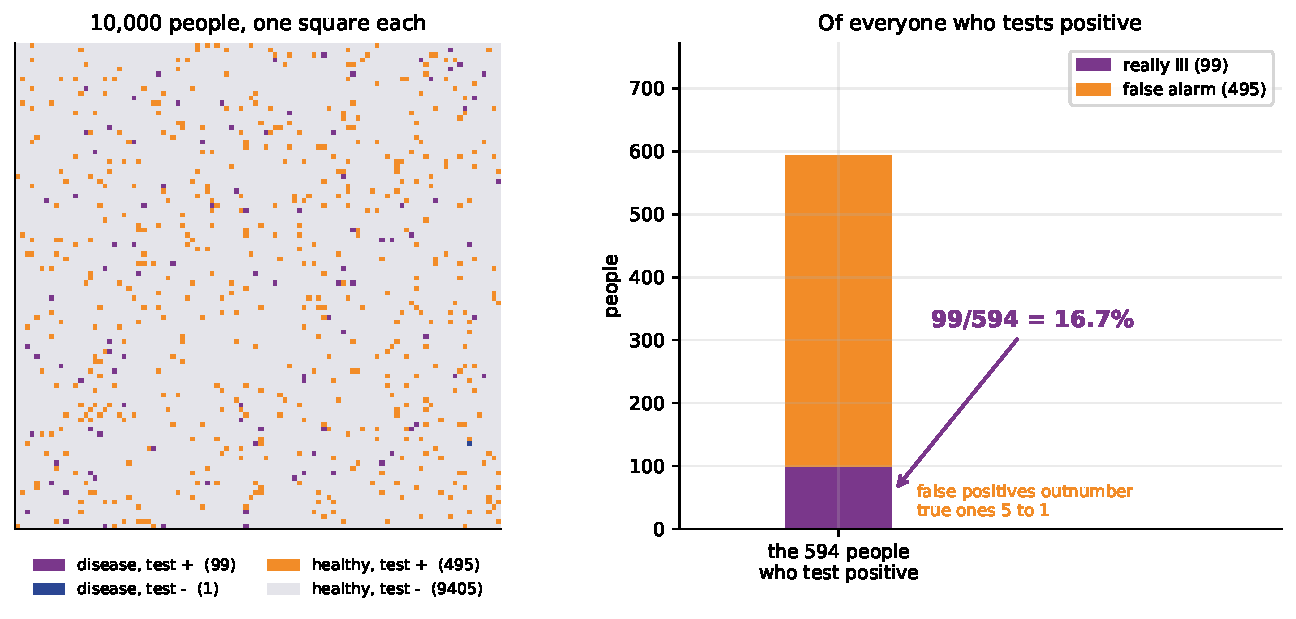
\includegraphics[width=0.94\textwidth]{basegrid.pdf}
\caption{Ten thousand people, one square each. Purple: ill and correctly
flagged ($99$). Blue: ill and missed ($1$). Orange: healthy and wrongly
flagged ($495$). Grey: healthy and correctly cleared ($9405$). The right-hand
bar keeps only the $594$ people who tested positive. The orange part of it is
what disappears when a test is described by its accuracy alone.}
\label{fig:basegrid}
\end{figure}

\paragraph{Way three: run it.}

\begin{lstlisting}
PREV, SENS, SPEC = 0.01, 0.99, 0.95
num = SENS * PREV                              # P(+, D)
den = SENS * PREV + (1 - SPEC) * (1 - PREV)    # P(+)
print(num / den)
\end{lstlisting}
\begin{codeout}
joint  P(+, D)    = P(+|D) P(D)       = 0.99 * 0.01 = 0.009900
joint  P(+, notD) = P(+|notD) P(notD) = 0.05 * 0.99 = 0.049500
evidence P(+)     = 0.009900 + 0.049500 = 0.059400
POSTERIOR P(D|+)  = 0.009900 / 0.059400 = 0.166667   = 16.6667%
exact fraction    = 99/594 = 1/6 ?  True
P(D|-)            = 0.00010632  = 0.01063%
\end{codeout}

And, because it is worth knowing that the algebra describes reality rather
than the other way round, simulate two million people.

\begin{lstlisting}
rng = np.random.default_rng(0)
M   = 2_000_000
dis = rng.random(M) < PREV
tst = np.where(dis, rng.random(M) < SENS, rng.random(M) < 1 - SPEC)
print(dis[tst].mean())
\end{lstlisting}
\begin{codeout}
confirmed by simulation, 2,000,000 people, seed 0
   simulated P(D|+) = 0.165611   analytic 0.166667   difference 0.001055
\end{codeout}

\begin{caution}[The base-rate fallacy, in one sentence]
The test's specification gives you $P(+ \mid D) = 0.99$. The question asks
for $P(D \mid +)$. \textbf{Those are different numbers, and the thing that
separates them is the prior.} Here there are $99$ healthy people for every
ill one, and the test fires wrongly on $5\%$ of them --- so most positives
come from the large healthy group.
\end{caution}

\subsection{What would make the test useful?}

The posterior has two levers, and it is worth knowing which one to pull.

\begin{lstlisting}
for pv in [0.001, 0.005, 0.01, 0.05, 0.10, 0.20, 0.50]:
    print(pv, SENS * pv / (SENS * pv + (1 - SPEC) * (1 - pv)))
\end{lstlisting}
\begin{codeout}
sweep: what would make the test useful?
   prevalence  P(D|+)
       0.001  0.0194
       0.005  0.0905
       0.010  0.1667
       0.050  0.5103
       0.100  0.6875
       0.200  0.8319
       0.500  0.9519
   specificity P(D|+)   (prevalence held at 1%)
      0.9000  0.0909
      0.9500  0.1667
      0.9900  0.5000
      0.9990  0.9091
      0.9999  0.9901
\end{codeout}

\begin{itemize}[leftmargin=*]
  \item \textbf{Raise the prior.} Test people who have symptoms rather than
    everybody. At $20\%$ prevalence the same test gives $0.8319$. This is
    why population screening and diagnostic testing are different problems
    even when the instrument is identical.
  \item \textbf{Raise the specificity} --- not the sensitivity. Going from
    $95\%$ to $99.9\%$ specificity takes the posterior from $0.1667$ to
    $0.9091$. On a rare condition, \emph{false positives are the entire
    problem}, and improving the detection rate hardly moves the answer.
\end{itemize}

\subsection{Yesterday's posterior is today's prior}
\label{sec:sequential}

Suppose the patient takes the test a second time, independently, and it is
positive again. Two equivalent calculations:

\begin{lstlisting}
p2  = (SENS**2 * PREV) / (SENS**2 * PREV + (1-SPEC)**2 * (1-PREV))
p1  = SENS * PREV / (SENS * PREV + (1-SPEC) * (1-PREV))    # first posterior
p2b = (SENS * p1)  / (SENS * p1  + (1-SPEC) * (1-p1))      # use it as a prior
\end{lstlisting}
\begin{codeout}
two independent positive tests (repeat the test)
   P(D|+,+) = 0.798387 = 79.84%
   sequential form: use the first posterior as the second prior
   P(D|+) then update again = 0.798387   same answer: True
\end{codeout}

\begin{keyidea}
The posterior after one observation \emph{is} the correct prior for the next.
You may absorb evidence all at once or one piece at a time and you will
arrive at the same number. That is what makes Bayes' theorem a rule for
\emph{updating} rather than a one-off calculation.
\end{keyidea}

\begin{figure}[htbp]
\centering
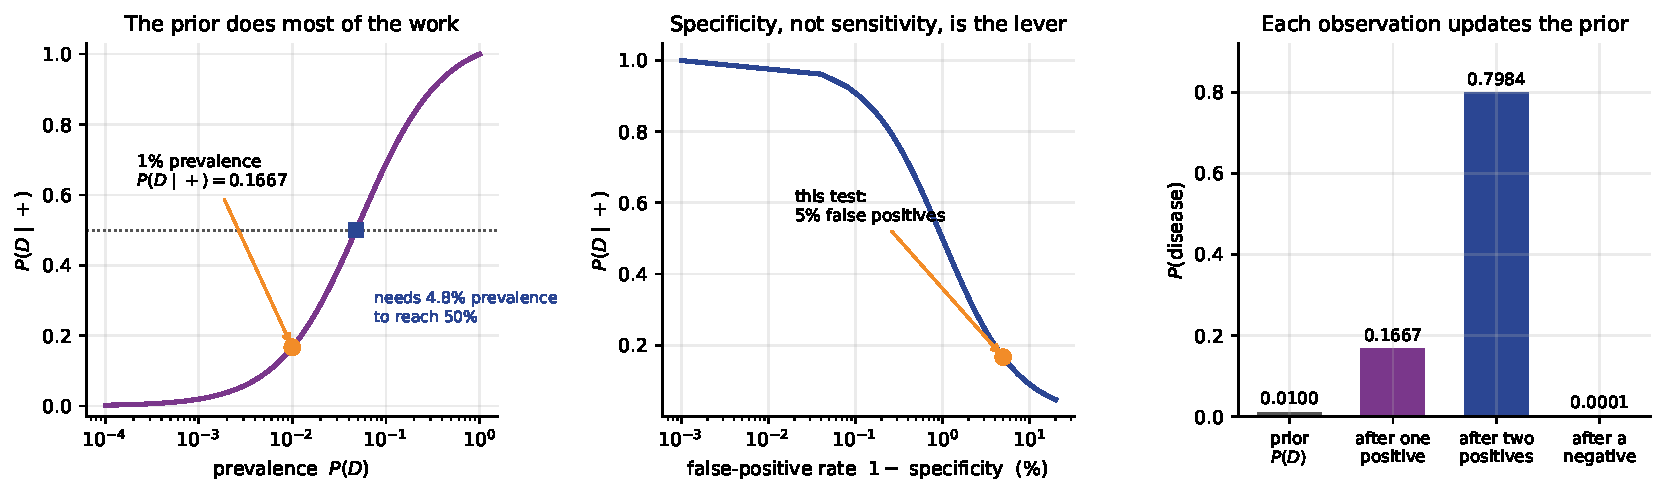
\includegraphics[width=\textwidth]{prevalence.pdf}
\caption{Left: the posterior as a function of prevalence; you need $4.8\%$
prevalence before a positive result is even an even-money bet. Centre: the
posterior against the false-positive rate --- the steep part of this curve is
where the money is. Right: sequential updating. Prior $0.0100$; after one
positive $0.1667$; after two $0.7984$; after a negative $0.0001$.}
\label{fig:prev}
\end{figure}

% =========================================================================
\section{Two decision rules: ML and MAP}
\label{sec:decide}

A classifier must eventually commit to a label. There are two natural rules,
and the difference between them is exactly the prior.

\begin{center}\small
\begin{tabular}{@{}llp{7.6cm}@{}}
\toprule
\textbf{Rule} & \textbf{Formula} & \textbf{Reads as}\\
\midrule
maximum likelihood (ML) & $\arg\max_c P(x \mid c)$ &
  which class best explains what I saw? Ignores how common the classes are.\\
maximum a posteriori (MAP) & $\arg\max_c P(x \mid c) P(c)$ &
  which class is most probable, given what I saw? This is what a classifier
  uses.\\
\bottomrule
\end{tabular}
\end{center}

They agree whenever the priors are equal, and they can disagree whenever they
are not. The medical test is the cleanest example there is.

\begin{codeout}
MAP against ML on the same evidence
   ML  rule: argmax P(+|c)      -> P(+|D)=0.9900 vs P(+|notD)=0.0500  -> says DISEASE
   MAP rule: argmax P(+|c)P(c)  -> 0.009900 vs 0.049500  -> says NO DISEASE
   the prior ratio is 99:1 against; the likelihood ratio is only 19.8:1 in favour
\end{codeout}

Read the last line slowly. A positive result is $19.8$ times more consistent
with disease than with health, which is genuinely strong evidence. It is not
strong enough, because it starts $99$ to $1$ behind.

\begin{keyidea}[The odds form, which is the whole of Bayesian updating]
\[
  \underbrace{\frac{P(D \mid +)}{P(\lnot D \mid +)}}_{\text{posterior odds}}
  \;=\;
  \underbrace{\frac{P(+ \mid D)}{P(+ \mid \lnot D)}}_{\text{likelihood ratio}}
  \;\times\;
  \underbrace{\frac{P(D)}{P(\lnot D)}}_{\text{prior odds}}
  \qquad\text{here}\qquad
  \frac{1}{5} = 19.8 \times \frac{1}{99}.
\]
The evidence $P(x)$ cancels, so this form needs no normalising at all. One
multiplication.
\end{keyidea}

\begin{caution}
``Maximum likelihood'' is used in two different senses in this course and you
must keep them apart. Here it is a \emph{decision rule} for choosing a class.
In Section~\ref{sec:gauss} it is an \emph{estimation} method for choosing
$\mu$ and $\sigma$. The word is the same; the object being maximised is not.
\end{caution}

% =========================================================================
\section{From Bayes' theorem to a classifier}
\label{sec:naive}

\subsection{The classifier writes itself, and then stops}

An instance is a vector of $d$ features, $x = (x_1, x_2, \ldots, x_d)$.
Applying MAP gives
\[
  \hat{c} \;=\; \arg\max_{c} \; P(c)\,P(x_1, x_2, \ldots, x_d \mid c).
\]
The prior is easy: count the classes. The likelihood is not. It is a
probability attached to \emph{every possible combination} of feature values.
With $d$ binary features that is a table of $2^d$ cells for each class, and
every cell must be estimated from data.

\subsection{Counting the parameters}
\label{sec:params}

\begin{lstlisting}
for d in [3, 5, 10, 20, 30, 64]:
    print(d, 2 * (2**d - 1), 2 * d)
\end{lstlisting}
\begin{codeout}
d binary features, 2 classes
    d        joint  C(2^d - 1)     naive  C*d            ratio
    3                       14              6                2
    5                       62             10                6
   10                    2,046             20              102
   20                2,097,150             40           52,429
   30            2,147,483,646             60       35,791,394
   64 36,893,488,147,419,103,230            128 288,230,376,151,711,744
\end{codeout}

\texttt{breast\_cancer} has $30$ features and $569$ patients. If those
features were binary, the joint table would have $2{,}147{,}483{,}646$ free
parameters --- roughly one training row for every four million parameters.
The situation is not merely difficult; it is arithmetically hopeless. A cell
never observed gets probability zero, and a cell observed once gets
probability $1/n$.

\begin{figure}[htbp]
\centering
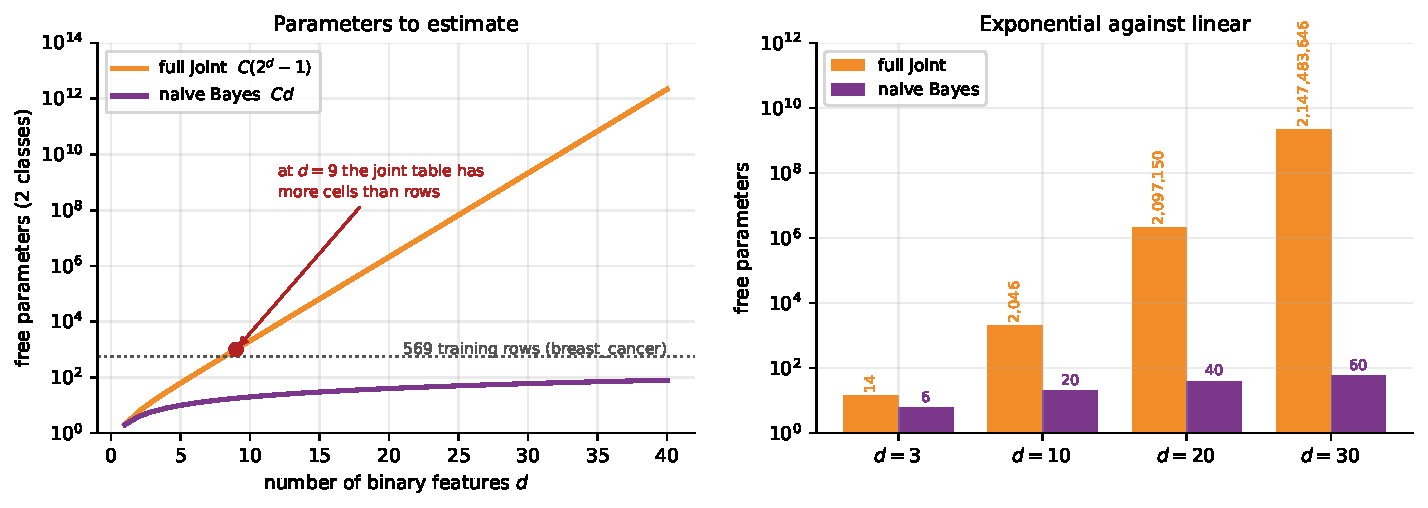
\includegraphics[width=\textwidth]{params.pdf}
\caption{Free parameters against the number of binary features, two classes.
The joint table crosses the $569$ rows of \texttt{breast\_cancer} at
$\mathbf{d = 9}$ --- nine binary features. Everything to the right of that
point is a model you cannot fit. The purple line is naive Bayes, which grows
linearly.}
\label{fig:params}
\end{figure}

\subsection{The naive assumption, stated precisely}
\label{sec:assumption}

\begin{keyidea}[Conditional independence given the class]
\[
  P(x_1, x_2, \ldots, x_d \mid c) \;=\; \prod_{j=1}^{d} P(x_j \mid c)
\]
Equivalently: $P(x_i \mid c, x_j) = P(x_i \mid c)$ for every $i \neq j$.
\textbf{Once you know the class}, knowing one feature tells you nothing more
about any other.
\end{keyidea}

Two things it does \emph{not} say, both of which are commonly written in
examination answers and both of which are wrong.

\begin{itemize}[leftmargin=*]
  \item It does not say the features are independent. \emph{Outlook} and
    \emph{humidity} are obviously related in the population; the assumption
    is only that they are unrelated \emph{within each class}.
  \item It does not say the features are irrelevant to each other. It says
    the class accounts for all of the relationship between them.
\end{itemize}

The assumption is almost always false. It is made anyway, and the reason is
purely arithmetic:

\begin{lstlisting}
cards = [3, 3, 2, 2]           # outlook, temperature, humidity, wind
print(2 * (np.prod(cards) - 1), 2 * sum(c - 1 for c in cards))
\end{lstlisting}
\begin{codeout}
the tennis table: outlook(3) temperature(3) humidity(2) wind(2), 2 classes
   full joint        70 free parameters (a 36-cell table per class)
   naive Bayes       12 free parameters + 1 for the prior
   training rows available: 14
   rows per joint cell on average: 0.194
\end{codeout}

Seventy free parameters against fourteen rows means $0.194$ rows per cell:
most cells of the joint table are empty. Twelve free parameters against
fourteen rows means every one is estimated from at least five rows.
\textbf{The trade is a wrong model you can fit against a right model you
cannot.}

\subsection{The complete algorithm}

Substituting the assumption into MAP gives the naive Bayes classifier:
\[
  \hat{c} \;=\; \arg\max_{c \in \mathcal{C}} \;
    P(c) \prod_{j=1}^{d} P(x_j \mid c).
\]

\begin{center}\small
\begin{tabular}{@{}lll@{}}
\toprule
\textbf{Quantity} & \textbf{Estimated as} & \textbf{scikit-learn class}\\
\midrule
$P(c)$ & $N_c / N$ & (all of them)\\
$P(x_j \mid c)$, categorical levels & $N_{tjc} / N_c$ &
  \texttt{CategoricalNB}\\
$P(x_j \mid c)$, word counts & $T_{cw} / \sum_{w'} T_{cw'}$ &
  \texttt{MultinomialNB}\\
$P(x_j \mid c)$, binary presence & Bernoulli per feature &
  \texttt{BernoulliNB}\\
$P(x_j \mid c)$, continuous & $\mathcal{N}(x_j; \mu_{jc}, \sigma^2_{jc})$ &
  \texttt{GaussianNB}\\
\bottomrule
\end{tabular}
\end{center}

\begin{keyidea}
\textbf{Training a naive Bayes classifier is counting.} There is no
iteration, no gradient, no loss surface and --- apart from the smoothing
constant --- no hyperparameter. One pass over the data accumulates every
statistic the model needs.
\end{keyidea}

% =========================================================================
\section{Naive Bayes worked entirely by hand}
\label{sec:hand}

The example below is the one every Indian syllabus uses, and the one the
class test will use. Learn to produce the whole thing in about four minutes.

\subsection{The training table}

\begin{center}\small
\begin{tabular}{@{}rllllc@{}}
\toprule
\# & Outlook & Temperature & Humidity & Wind & \textbf{Play}\\
\midrule
1 & Sunny & Hot & High & Weak & No\\
2 & Sunny & Hot & High & Strong & No\\
3 & Overcast & Hot & High & Weak & Yes\\
4 & Rain & Mild & High & Weak & Yes\\
5 & Rain & Cool & Normal & Weak & Yes\\
6 & Rain & Cool & Normal & Strong & No\\
7 & Overcast & Cool & Normal & Strong & Yes\\
8 & Sunny & Mild & High & Weak & No\\
9 & Sunny & Cool & Normal & Weak & Yes\\
10 & Rain & Mild & Normal & Weak & Yes\\
11 & Sunny & Mild & Normal & Strong & Yes\\
12 & Overcast & Mild & High & Strong & Yes\\
13 & Overcast & Hot & Normal & Weak & Yes\\
14 & Rain & Mild & High & Strong & No\\
\bottomrule
\end{tabular}
\end{center}

Nine \emph{Yes} and five \emph{No}, so the priors are
\[
  P(\text{Yes}) = \tfrac{9}{14} = 0.642857, \qquad
  P(\text{No})  = \tfrac{5}{14} = 0.357143.
\]

\subsection{Step 1 --- the conditional probability tables}

For each feature and each level, count how often that level occurs among the
nine \emph{Yes} days and among the five \emph{No} days.

\begin{center}\small
\begin{tabular}{@{}llrlrl@{}}
\toprule
\textbf{Feature} & \textbf{Level} & \multicolumn{2}{c}{\textbf{given Yes}
  ($N_c = 9$)} & \multicolumn{2}{c}{\textbf{given No} ($N_c = 5$)}\\
\midrule
Outlook & Overcast & 4/9 & $=0.4444$ & \textbf{0/5} & $=\mathbf{0.0000}$\\
        & Rain     & 3/9 & $=0.3333$ & 2/5 & $=0.4000$\\
        & Sunny    & 2/9 & $=0.2222$ & 3/5 & $=0.6000$\\
\midrule
Temperature & Cool & 3/9 & $=0.3333$ & 1/5 & $=0.2000$\\
            & Hot  & 2/9 & $=0.2222$ & 2/5 & $=0.4000$\\
            & Mild & 4/9 & $=0.4444$ & 2/5 & $=0.4000$\\
\midrule
Humidity & High   & 3/9 & $=0.3333$ & 4/5 & $=0.8000$\\
         & Normal & 6/9 & $=0.6667$ & 1/5 & $=0.2000$\\
\midrule
Wind & Strong & 3/9 & $=0.3333$ & 3/5 & $=0.6000$\\
     & Weak   & 6/9 & $=0.6667$ & 2/5 & $=0.4000$\\
\bottomrule
\end{tabular}
\end{center}

Each block sums to $1$ down its column, which is a free check. \textbf{This
table is the entire trained model.} Twelve free numbers and a prior. Note the
bold zero; Section~\ref{sec:zero} is about it.

\subsection{Step 2 --- classify a new day}

\begin{worked}[$x = (\text{Sunny}, \text{Cool}, \text{High},
\text{Strong})$]
Multiply the prior by the four conditional probabilities, once for each
class.
\begin{align*}
  \text{score}(\text{No})
    &= \tfrac{5}{14} \times \tfrac{3}{5} \times \tfrac{1}{5}
       \times \tfrac{4}{5} \times \tfrac{3}{5}\\
    &= 0.357143 \times 0.6 \times 0.2 \times 0.8 \times 0.6
     = \mathbf{0.02057143}\\[0.4em]
  \text{score}(\text{Yes})
    &= \tfrac{9}{14} \times \tfrac{2}{9} \times \tfrac{3}{9}
       \times \tfrac{3}{9} \times \tfrac{3}{9}\\
    &= 0.642857 \times 0.222222 \times 0.333333^{3}
     = \mathbf{0.00529101}
\end{align*}
These are not probabilities: they are $P(c)P(x \mid c)$, and they do not sum
to one. Their sum \emph{is} the evidence:
\[
  P(x) = 0.02057143 + 0.00529101 = 0.02586243 .
\]
Divide to normalise:
\[
  P(\text{No} \mid x) = \frac{0.02057143}{0.02586243} = \mathbf{0.795417},
  \qquad
  P(\text{Yes} \mid x) = \frac{0.00529101}{0.02586243} = \mathbf{0.204583}.
\]
\textbf{Prediction: \emph{No}}, at posterior odds of $3.8880$ to $1$.
\end{worked}

Five multiplications and one division. If the question asks only for the
label you can stop before the division; if it asks for a probability you
cannot.

\begin{figure}[htbp]
\centering
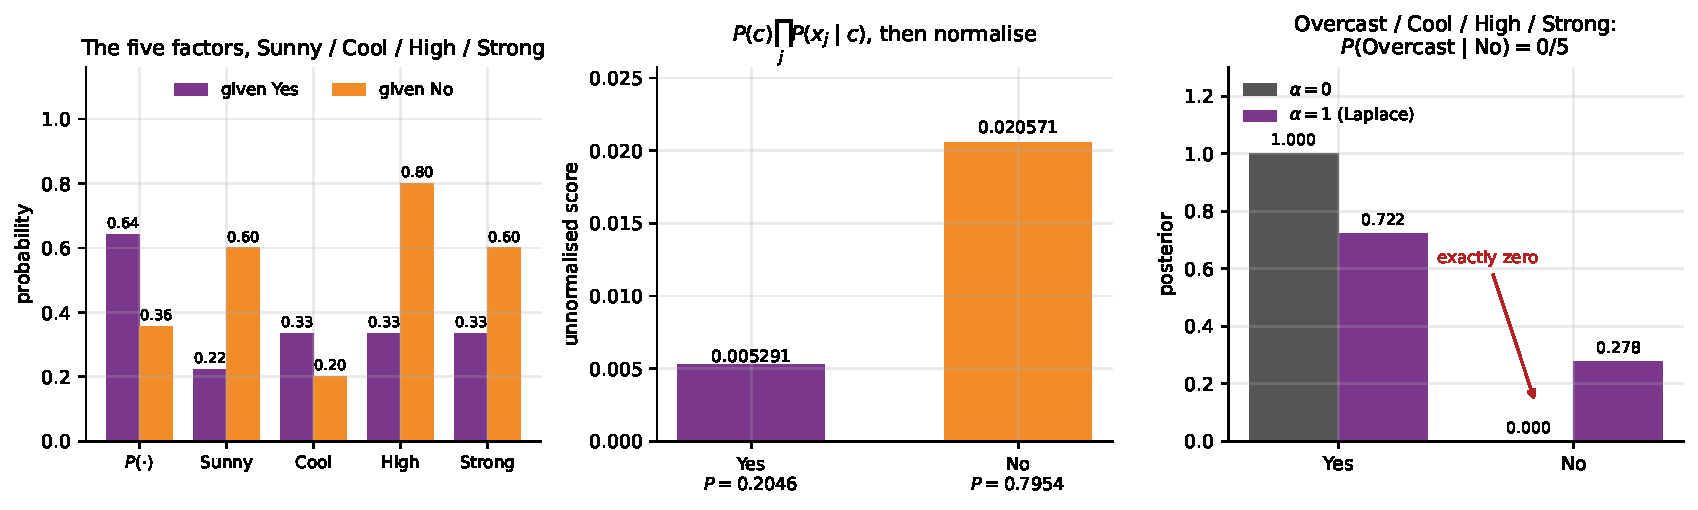
\includegraphics[width=\textwidth]{tennis.pdf}
\caption{Left: the five factors that get multiplied. \emph{High} humidity is
the strongest single piece of evidence against playing, $0.80$ against
$0.33$. Centre: the two unnormalised scores, before dividing by the evidence.
Right: what happens to the same instance with \emph{Overcast} substituted for
\emph{Sunny} --- the subject of Section~\ref{sec:zero}.}
\label{fig:tennis}
\end{figure}

\subsection{The same thing in scikit-learn}

\texttt{CategoricalNB} expects integer-coded levels, so encode first. The
$\alpha$ argument is smoothing; set it to almost zero to reproduce the raw
counting above.

\begin{lstlisting}
from sklearn.naive_bayes import CategoricalNB
from sklearn.preprocessing import OrdinalEncoder

LEVELS = [["Overcast","Rain","Sunny"], ["Cool","Hot","Mild"],
          ["High","Normal"], ["Strong","Weak"]]
enc  = OrdinalEncoder(categories=LEVELS)
Xe   = enc.fit_transform(np.array(X_t, dtype=object))
cnb0 = CategoricalNB(alpha=1e-10, force_alpha=True).fit(Xe, ye)
q    = enc.transform(np.array([("Sunny","Cool","High","Strong")], dtype=object))
print(cnb0.predict_proba(q))
\end{lstlisting}
\begin{codeout}
the same instance through sklearn CategoricalNB(alpha=1e-10)
      predict_proba  No 0.795417   Yes 0.204583
      predict        No
      agrees with the hand calculation to 7.68e-12
\end{codeout}

\begin{codeout}
resubstitution accuracy of the hand model on all 14 rows
      13/14 = 0.9286
\end{codeout}

\begin{keyidea}
There is nothing inside \texttt{CategoricalNB} that you did not just do with
a pen. The only surprise is $\alpha$: the library smooths by default, and to
reproduce textbook arithmetic you must switch it off. The next section is why
the default exists.
\end{keyidea}

\begin{tryit}
Change the query to $(\text{Rain}, \text{Mild}, \text{Normal},
\text{Weak})$ and work it out by hand before running it. You should get
$\text{score}(\text{Yes}) = \tfrac{9}{14}\cdot\tfrac{3}{9}\cdot\tfrac{4}{9}
\cdot\tfrac{6}{9}\cdot\tfrac{6}{9} = 0.028219$ and
$\text{score}(\text{No}) = \tfrac{5}{14}\cdot\tfrac{2}{5}\cdot\tfrac{2}{5}
\cdot\tfrac{1}{5}\cdot\tfrac{2}{5} = 0.004571$, giving
$P(\text{Yes} \mid x) = 0.860577$.
\end{tryit}

% =========================================================================
\section{The zero-frequency problem and Laplace smoothing}
\label{sec:zero}

\subsection{One empty cell destroys the product}

Look again at the conditional probability table. \emph{Overcast} never
appears with \emph{No}: all four overcast days were played. So
\[
  P(\text{Overcast} \mid \text{No}) = \tfrac{0}{5} = 0 .
\]
Now classify $x = (\text{Overcast}, \text{Cool}, \text{High},
\text{Strong})$. Three of the four features favour \emph{No}: high humidity
($0.80$ against $0.33$), strong wind ($0.60$ against $0.33$), and cool is
close to neutral.

\begin{codeout}
classify ('Overcast', 'Cool', 'High', 'Strong') with alpha = 0
      P(No) * prod = 5/14 * 0/5 * 1/5 * 4/5 * 3/5 = 0.00000000
      P(Yes) * prod = 9/14 * 4/9 * 3/9 * 3/9 * 3/9 = 0.01058201
      P(Yes|x) = 1.000000   P(No|x) = 0.000000
      the model says 'No' is IMPOSSIBLE -- probability exactly zero,
      even though three of the four features point at No.
      the other three factors for No were 1/5, 4/5, 3/5 -- none of them small.
\end{codeout}

\begin{caution}[A probability of exactly zero is a claim you cannot defend]
The model is not saying ``unlikely''. It is saying \textbf{impossible}: no
amount of evidence from the other features can recover the class, because
everything is multiplied by $0$. One unobserved combination has vetoed an
entire class, and the sample size behind that veto is \emph{five rows}.
Multiplication is unforgiving in a way that addition is not.
\end{caution}

\subsection{The fix}

\begin{keyidea}[Laplace, or add-one, smoothing]
\[
  \hat{P}(x_j = t \mid c) \;=\; \frac{N_{tjc} + \alpha}{N_c + \alpha\,n_j}
\]
where $n_j$ is the number of \emph{levels} feature $j$ has. Add $\alpha$ to
the numerator and $\alpha n_j$ to the denominator, so the estimates still sum
to one down the column. $\alpha = 1$ is \emph{Laplace} smoothing;
$0 < \alpha < 1$ is \emph{Lidstone} smoothing.
\end{keyidea}

\emph{Outlook} has three levels, so for the five \emph{No} days the
denominator becomes $5 + 3 = 8$:
\[
  P(\text{Overcast} \mid \text{No}) = \frac{0 + 1}{5 + 3} = \frac{1}{8}
    = 0.1250 .
\]

\begin{caution}
The single commonest examination error on this topic is using the wrong
denominator --- adding $1$ to the numerator and $1$ to the denominator, or
adding the number of \emph{classes} rather than the number of \emph{levels}.
For the tennis table with $\alpha = 1$: \texttt{Outlook} and
\texttt{Temperature} have three levels, so \emph{No} denominators are
$5 + 3 = 8$ and \emph{Yes} denominators are $9 + 3 = 12$; \texttt{Humidity}
and \texttt{Wind} have two levels, so $5 + 2 = 7$ and $9 + 2 = 11$.
\end{caution}

\subsection{Before and after, with numbers}

\begin{codeout}
the same instance with Laplace alpha = 1
      P(No) * prod = 5/14 * 1/8 * 2/8 * 5/7 * 4/7 = 0.00455539
      P(Yes) * prod = 9/14 * 5/12 * 4/12 * 4/11 * 4/11 = 0.01180638
      P(Overcast|No) = (0+1)/(5+3) = 0.1250
      P(Yes|x) = 0.721583   P(No|x) = 0.278417
      'impossible' has become 27.84%
\end{codeout}

\begin{center}\small
\begin{tabular}{@{}lcc@{}}
\toprule
 & $P(\text{No} \mid x)$ & $P(\text{Yes} \mid x)$\\
\midrule
$\alpha = 0$ & $\mathbf{0.000000}$ & $1.000000$\\
$\alpha = 1$ & $\mathbf{0.278417}$ & $0.721583$\\
\bottomrule
\end{tabular}
\end{center}

Every fraction on that first output line can be read straight off the level
counts, and you should check that you can.

\subsection{How much smoothing?}

\begin{codeout}
alpha sweep on the same instance
      alpha    P(No|x)   P(Yes|x)  prediction
       0.00   0.000000   1.000000  Yes
       0.01   0.006403   0.993597  Yes
       0.10   0.057749   0.942251  Yes
       0.50   0.197785   0.802215  Yes
       1.00   0.278417   0.721583  Yes
       2.00   0.340932   0.659068  Yes
       5.00   0.375650   0.624350  Yes
      20.00   0.370805   0.629195  Yes
     100.00   0.360719   0.639281  Yes
   as alpha grows the conditionals wash out and the PRIOR takes over:
   P(Yes) = 9/14 = 0.6429, which is the limit above
\end{codeout}

$\alpha$ interpolates between two extremes. At $\alpha \to 0$ the model
trusts the counts completely, including the accidental zeros. At
$\alpha \to \infty$ every conditional probability tends to $1/n_j$, the
factors become identical for every class, and the posterior tends to the
prior --- $9/14 = 0.6429$, which is exactly what the last rows of the table
show. \textbf{It is a regularisation parameter and should be
cross-validated like any other.}

\begin{figure}[htbp]
\centering
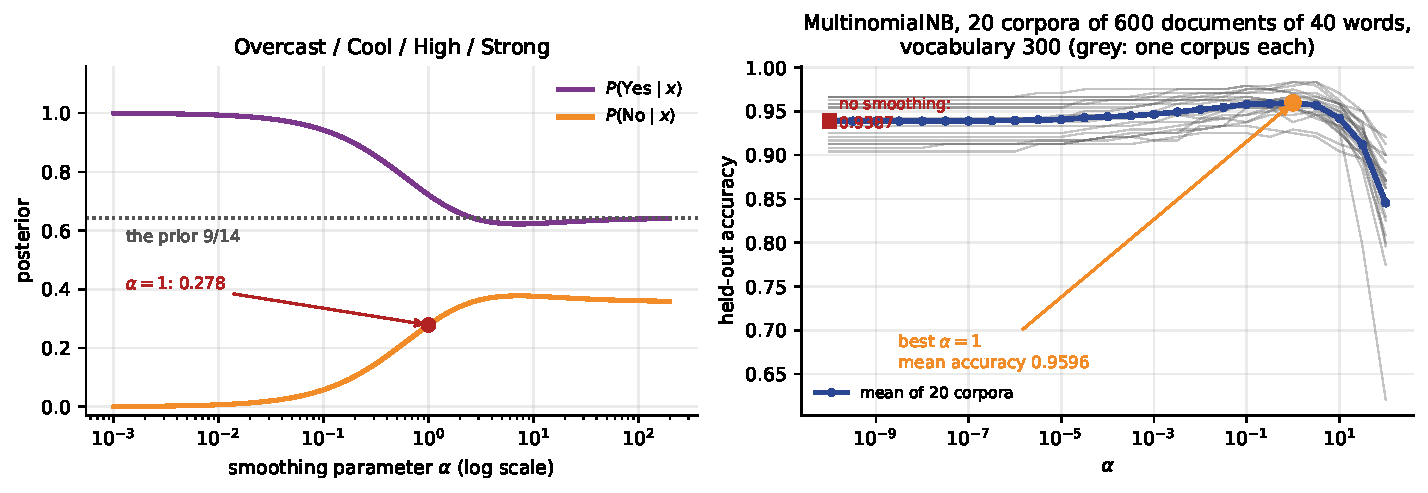
\includegraphics[width=\textwidth]{smoothing.pdf}
\caption{Left: the tennis posterior as $\alpha$ sweeps from $0$ to $200$,
starting at the indefensible $0$ and flattening onto the prior $9/14$. Right:
held-out accuracy of \texttt{MultinomialNB}, averaged over \emph{twenty}
corpora of $600$ synthetic documents of $40$ words over a vocabulary of $300$
(the individual corpora are the grey lines). No smoothing scores $0.9387$;
the best $\alpha$, which is $1$, scores $0.9596$; $\alpha = 100$ falls to
$0.8454$. Too much smoothing costs more than too little --- and one corpus
alone would not have told you either thing.}
\label{fig:smoothing}
\end{figure}

\subsection{Reported honestly: on this table the label never flips}

It would be convenient to claim that smoothing rescues the prediction. On
these fourteen rows it does not, and saying so would be inventing a result.

\begin{codeout}
how many of the 36 possible days contain a zero, and how many flip?
   36 possible days; 12 of them make one class exactly impossible (33.3%)
   smoothing changes the prediction on 0 of the 36
mean |change| in P(Yes|x) across all 36 days when alpha goes 0 -> 1
   mean 0.0942   max 0.4356
\end{codeout}

A third of all possible days drive one class to exactly zero. But every zero
in this table falls on \emph{Overcast} given \emph{No} --- the minority class,
which was losing anyway --- so the \emph{argmax} never changes. What
smoothing fixes here is the posterior: on average it moves
$P(\text{Yes} \mid x)$ by $0.0942$, and at worst by $0.4356$.

\textbf{On other tables the label does flip.} Practice question~3 uses a
ten-row table on which $\alpha = 0$ predicts \emph{No} at $0.529412$ and
$\alpha = 1$ predicts \emph{Yes} at $0.531453$ --- for the same instance. And
on text it is worse than a flip, as the next section shows: there the zeros
land on \emph{both} classes at once and the model has no opinion at all.

% =========================================================================
\section{Text, log-probabilities and underflow}
\label{sec:logs}

\subsection{A twelve-message corpus, written out inline}

Naive Bayes' historical claim to fame is spam filtering, so we need a text
corpus. Because the campus network blocks
\texttt{fetch\_20newsgroups}, here is one typed out in the source.

\begin{lstlisting}
SPAM = ["win a free laptop click this link now",
        "congratulations you win a free prize click now",
        "free money click the link to claim your prize",
        "urgent claim your free gift click here now",
        "you win cash prize click link urgent",
        "free free free click now win big money"]
HAM  = ["the lecture notes for the machine learning class are on the portal",
        "please submit your assignment before the deadline on friday",
        "the lab session is moved to the afternoon slot",
        "can you send me the notes from the lecture",
        "the exam schedule for the class is on the portal now",
        "your assignment feedback is ready please collect it"]
vec = CountVectorizer()
X   = vec.fit_transform(SPAM + HAM).toarray()
\end{lstlisting}
\begin{codeout}
12 messages (6 spam, 6 ham), vocabulary of 51 words
total word tokens: spam 46, ham 58
\end{codeout}

For text the natural model is \texttt{MultinomialNB}: a document is a bag of
word counts, and
\[
  \hat{P}(w \mid c) = \frac{T_{cw} + \alpha}
                           {\bigl(\sum_{w'} T_{cw'}\bigr) + \alpha V}
\]
where $T_{cw}$ is how many times word $w$ occurs across all documents of
class $c$, and $V$ is the vocabulary size. Note the denominator: it is the
\emph{token} count for the class, not the document count, plus $\alpha V$.

\begin{codeout}
the most discriminative words (Laplace alpha = 1)
   word             n(spam)  n(ham)    P(w|S)    P(w|H)  log ratio
   free                   7       0   0.08247   0.00917     2.1961
   click                  6       0   0.07216   0.00917     2.0625
   win                    4       0   0.05155   0.00917     1.7261
   link                   3       0   0.04124   0.00917     1.5029
   prize                  3       0   0.04124   0.00917     1.5029
   urgent                 2       0   0.03093   0.00917     1.2152
   notes                  0       2   0.01031   0.02752    -0.9820
   is                     0       3   0.01031   0.03670    -1.2697
   on                     0       3   0.01031   0.03670    -1.2697
   the                    1      11   0.02062   0.11009    -1.6751
\end{codeout}

Check one entry by hand: $P(\text{free} \mid S) = (7+1)/(46+51) = 8/97
= 0.08247$ and $P(\text{free} \mid H) = (0+1)/(58+51) = 1/109 = 0.00917$.

\subsection{Scoring a message with logs}

\begin{worked}[``click the free link'']
Take the logarithm of $P(c)\prod_w P(w \mid c)$. The product becomes a sum.
\begin{codeout}
      log P(S)  = log 0.5000 = -0.693147
      log P(H)  = log 0.5000 = -0.693147
      click    P(w|S)=0.07216 log=-2.6288   P(w|H)=0.00917 log=-4.6913
      free     P(w|S)=0.08247 log=-2.4953   P(w|H)=0.00917 log=-4.6913
      link     P(w|S)=0.04124 log=-3.1884   P(w|H)=0.00917 log=-4.6913
      the      P(w|S)=0.02062 log=-3.8816   P(w|H)=0.11009 log=-2.2064
      total log score  spam -12.887198   ham -16.973632
      P(spam|msg) = 0.983479   P(ham|msg) = 0.016521
\end{codeout}
The margin is $-12.887198 - (-16.973632) = 4.086434$, and for two classes
the posterior is a logistic function of the margin:
$1/(1 + e^{-4.086434}) = 0.983479$. Note that ``the'' argues for ham and
loses three to one.
\end{worked}

\begin{codeout}
   sklearn MultinomialNB(alpha=1)  ham 0.016521  spam 0.983479
   agreement to 8.88e-16
\end{codeout}

\begin{figure}[htbp]
\centering
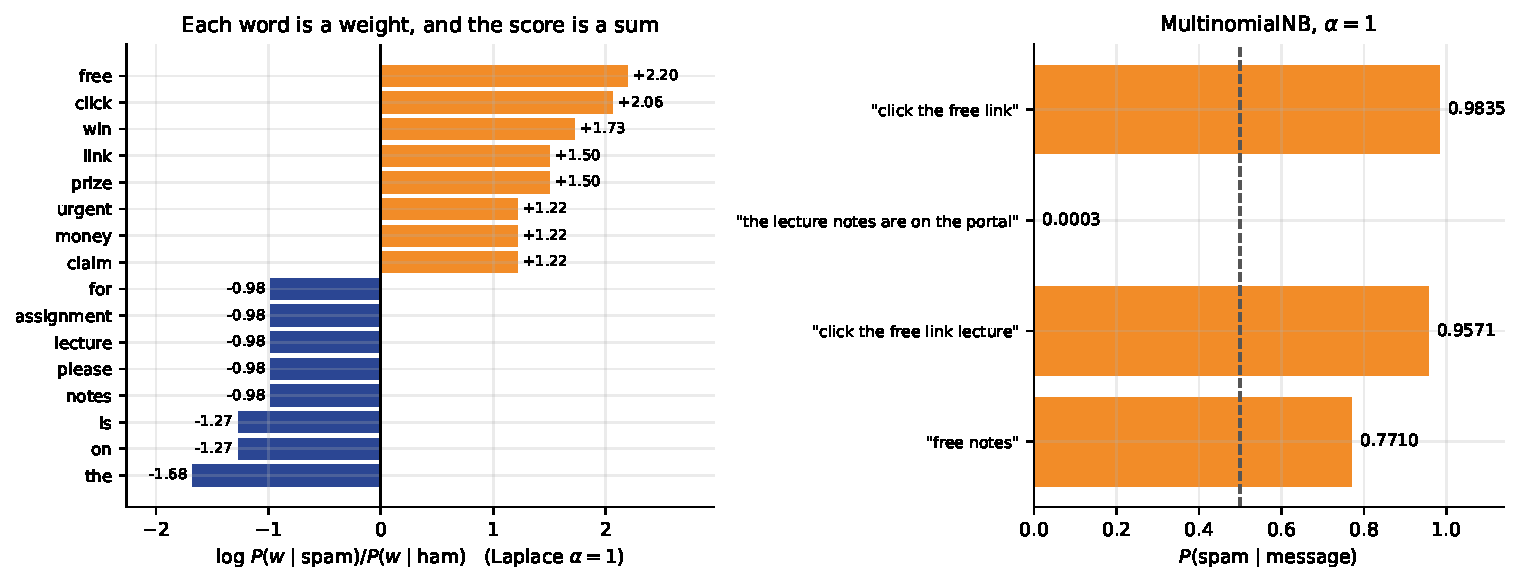
\includegraphics[width=\textwidth]{spam.pdf}
\caption{Left: $\log P(w \mid S)/P(w \mid H)$ for the sixteen most
opinionated words in the corpus. Each word is a weight and classification is
addition. Right: four messages scored. ``Click the free link lecture'' still
scores $0.9571$ --- one ham word cannot overturn three spam words, which is
exactly what summing evidence should do.}
\label{fig:spam}
\end{figure}

\subsection{Why logs are not optional}

The reason is not elegance. It is that the product does not fit in a
floating-point number.

\begin{codeout}
float64 limits
   smallest normal    2.2251e-308
   smallest subnormal 4.9407e-324
   1e-200 * 1e-200 =  0.0000e+00
\end{codeout}

Build a realistic corpus --- $600$ synthetic documents of $120$ tokens over a
vocabulary of $400$, two classes sharing $88\%$ of their vocabulary --- fit
\texttt{MultinomialNB}, and then multiply one document's per-token
probabilities together, one token at a time.

\begin{lstlisting}
pw   = np.exp(m.feature_log_prob_)      # P(word | class)
toks = np.repeat(np.arange(VOC), Xte[0])
p = 1.0
for t in toks:
    p *= pw[1, t]
\end{lstlisting}
\begin{codeout}
   MultinomialNB test accuracy 0.9722
   per-word probabilities: min 3.888e-05  median 1.256e-03  max 2.963e-02

     tokens      raw product      sum of logs       exp(sum)
          1     6.868132e-03          -4.9809   6.868132e-03
          5     3.225750e-13         -28.7624   3.225750e-13
         10     4.554564e-23         -51.4433   4.554564e-23
         20     2.625046e-41         -93.4409   2.625046e-41
         50    5.555479e-107        -244.6618  5.555479e-107
        100    7.423356e-226        -518.3796  7.423356e-226
        120    2.511950e-270        -620.7769  2.511950e-270
        200     0.000000e+00       -1023.0046   0.000000e+00
        400     0.000000e+00       -2050.9589   0.000000e+00
   the raw product first becomes EXACTLY 0.0 at 148 tokens
   a real e-mail is routinely longer than that
\end{codeout}

\textbf{One hundred and forty-eight tokens.} About one short paragraph. A
real e-mail, a product review or a support ticket is longer than that, and the
sum-of-logs column keeps working past $400$ tokens at $-2051.0$, which is
$\log(10^{-891})$ --- a number no floating-point format can represent, being
computed without difficulty.

\begin{figure}[htbp]
\centering
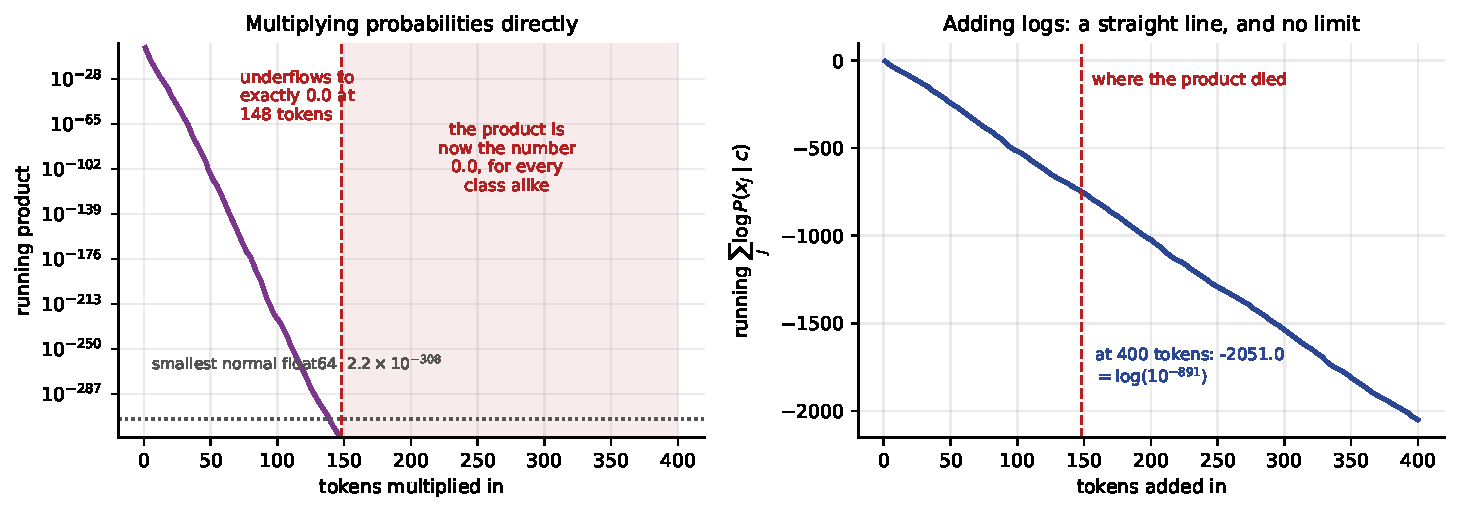
\includegraphics[width=\textwidth]{underflow.pdf}
\caption{Left: the running product on a logarithmic axis, falling off the
bottom of \texttt{float64} at token $148$; the shaded region is where the
number is literally $0.0$. Right: the same computation as a running sum of
logarithms --- a straight line with no floor at all.}
\label{fig:underflow}
\end{figure}

\subsection{And it is not a cosmetic problem}

Score the whole test set twice, once by multiplying and once by adding
logarithms, lengthening the documents by tiling the way an e-mail thread
grows.

\begin{codeout}
    tokens  both scores 0.0  one score 0.0  raw-product acc  log acc
       120                0              0           0.9722   0.9722
       240              180              0           0.5056   0.9722
       360              180              0           0.5056   0.9722
       480              180              0           0.5056   0.9722
   when both scores hit 0.0 the comparison is 0 > 0, which is False,
   so every one of those documents is silently assigned to class 0
\end{codeout}

\begin{caution}
At $240$ tokens \emph{all} $180$ test documents have both class scores equal
to $0.0$. The comparison \texttt{0.0 > 0.0} is \texttt{False}, so every
document is assigned to class $0$, the accuracy falls from $0.9722$ to
$0.5056$, and \textbf{nothing raises an error}. Be suspicious of any product
of more than about a hundred probabilities.
\end{caution}

\subsection{Getting back to a probability: log-sum-exp}

The argmax needs only the log scores. If you want a posterior that sums to
one you must exponentiate, and doing that naively re-creates the problem you
just solved.

\begin{lstlisting}
a = np.array([-800.0, -802.0])
print(np.log(np.exp(a).sum()))                      # naive
print(a.max() + np.log(np.exp(a - a.max()).sum()))  # stable
\end{lstlisting}
\begin{codeout}
   logs [-800. -802.]
   naive  exp(a).sum() = 0.0000e+00  -> log = -inf
   stable mx + log(sum(exp(a-mx))) = -799.873072
\end{codeout}

\begin{keyidea}[The log-sum-exp identity]
\[
  \log \sum_k e^{a_k} \;=\; a_{\max} + \log \sum_k e^{\,a_k - a_{\max}}
\]
Subtracting the maximum makes the largest exponent exactly $e^0 = 1$, so
nothing overflows and the dominant term never underflows. The identity is
exact, not an approximation --- it is only
$\log\bigl(e^{a_{\max}}\sum_k e^{a_k - a_{\max}}\bigr)$ expanded.
Use \texttt{scipy.special.logsumexp}.
\end{keyidea}

This is the same trick that makes \texttt{softmax} numerically safe in every
neural-network library, and you will meet it again in the neural-networks
lecture.

\subsection{How often is a word unseen? Count it}

The reason smoothing matters more on text than on the tennis table is
sparsity.

\begin{codeout}
5b. how often is a word unseen for one class? count it
   of the 51 words in the vocabulary, only 5 appear in BOTH classes
   31 are never seen in spam, 15 are never seen in ham
   so at alpha = 0 almost every message drives at least one class to exactly zero:
      "the lecture notes are free"    alpha=0: both zero      alpha=1: P(spam) = 0.1172
      "click the free link"           alpha=0: ham zero       alpha=1: P(spam) = 0.9835
      "the free portal"               alpha=0: both zero      alpha=1: P(spam) = 0.3867
      "win the exam"                  alpha=0: both zero      alpha=1: P(spam) = 0.3716
\end{codeout}

Five words out of fifty-one appear in both classes. Without smoothing, three
of those four test messages give \emph{both} classes a score of exactly zero
--- the model has no opinion whatever and the tie is broken by array order.
Measured on the larger corpus:

\begin{codeout}
5c. the same effect measured on a larger corpus (600 synthetic documents)
        alpha   test accuracy   labels changed vs alpha=1
        1e-10          0.9625                           6
       0.0001          0.9625                           6
         0.01          0.9625                           6
          0.1          0.9583                           5
            1          0.9542                           0
           10          0.9250                           9
\end{codeout}

On \emph{this} corpus the tiniest $\alpha$ wins and smoothing costs a little
accuracy --- which is the opposite of the point about to be made, so do not
take one corpus of $600$ documents as evidence. Draw twenty of them.

\begin{lstlisting}
def corpus(seed):                        # seed = 0, 1, 2, ... derived from SEED
    g = np.random.default_rng(seed)
    ...                                  # 600 documents, 40 words, vocab 300
for k in range(20):
    X, y = corpus(0 + k)
\end{lstlisting}
\begin{codeout}
        alpha   mean accuracy   worst corpus   best corpus
        1e-10          0.9387         0.9042        0.9667
       0.0001          0.9437         0.9125        0.9750
         0.01          0.9521         0.9250        0.9750
          0.1          0.9579         0.9250        0.9792
            1          0.9596         0.9250        0.9833
           10          0.9421         0.9042        0.9708
\end{codeout}

Now the shape is unmistakable and it is the shape you should remember: a rise
from $0.9387$ at effectively no smoothing to $0.9596$ at $\alpha = 1$, then a
fall to $0.9421$ at $\alpha = 10$. \textbf{Two points of accuracy, bought
with one added count per cell} --- and two more points lost if you add ten.
Any single corpus can and does sit anywhere in the $0.90$ to $0.98$ band, so
never tune $\alpha$ on one split and believe the answer.

One more distinction, because the table invites the wrong reading.
$\alpha = 10^{-10}$ is \emph{not} $\alpha = 0$; it is smoothing, just very
little of it, and nothing it produces is ever exactly zero. $\alpha = 0$ is a
different object altogether, and Section~\ref{sec:zero} has already shown
what it does: a hard zero, an undefined comparison and a label chosen by array
order.

% =========================================================================
\section{Gaussian naive Bayes: continuous features}
\label{sec:gauss}

\subsection{You cannot count a real number}

\emph{Petal width} $= 1.7$\,cm appears in the training set either zero times
or once. Counting gives $0$ or $1/50$, and neither is useful. The standard
answer is to stop counting and model the \emph{density} instead:
\[
  P(x_j \mid c) \;=\; \frac{1}{\sqrt{2\pi\sigma_{jc}^{2}}}
    \exp\!\left(-\frac{(x_j - \mu_{jc})^{2}}{2\sigma_{jc}^{2}}\right),
\]
with $\mu_{jc}$ and $\sigma^2_{jc}$ the ordinary sample mean and sample
variance of feature $j$ among the training rows of class $c$. Two numbers
per feature per class replace a whole histogram.

\begin{caution}
$P(x_j \mid c)$ is now a probability \emph{density}, and a density may exceed
$1$ --- look at the numbers below, where $p(1.5 \mid \text{versicolor}) =
1.372866$. That is legal. Densities are not probabilities; only their
integrals are. The values normalise away when you divide by the evidence.
\end{caution}

\subsection{By hand, on one iris measurement}

\begin{codeout}
load_iris, petal width (cm), by class
   class          n      mean   sd (ML)
   setosa        50    0.2460    0.1043
   versicolor    50    1.3260    0.1958
   virginica     50    2.0260    0.2719
\end{codeout}

\begin{worked}[A flower with petal width $1.7$\,cm]
Substitute into the density for each class. For \emph{virginica},
$\mu = 2.0260$ and $\sigma = 0.2719$:
\[
  p(1.7 \mid \text{virginica})
    = \frac{1}{0.2719\sqrt{2\pi}}
      \exp\!\left(-\frac{(1.7 - 2.0260)^2}{2 \times 0.2719^2}\right)
    = 0.7150527 .
\]
The three classes have $50$ rows each, so the priors are equal and the
posterior is just the densities normalised.
\begin{codeout}
   a flower with petal width 1.7 cm
      p(x|setosa     ) = 2.533257e-42   P(setosa|x) = 0.000000
      p(x|versicolor ) = 3.285675e-01   P(versicolor|x) = 0.314834
      p(x|virginica  ) = 7.150527e-01   P(virginica|x) = 0.685166
      PREDICTION: virginica
\end{codeout}
$0.7150527 / (0.7150527 + 0.3285675 + 2.5\times10^{-42}) = 0.685166$.
\end{worked}

\begin{codeout}
   sklearn GaussianNB on the single column
      theta_ (means)  [0.246 1.326 2.026]
      var_            [0.0109 0.0383 0.0739]
      sd              [0.1043 0.1958 0.2719]
      predict_proba(1.7) [0.     0.3148 0.6852]
      note var_ carries sklearn's var_smoothing of 3.096e-09

   the two decision boundaries, solved numerically
      boundaries at petal width [0.6333 1.6437] cm
\end{codeout}

The two boundaries at $0.6333$ and $1.6437$\,cm are where the posterior
curves cross. Note that they are \emph{not} halfway between the means:
because the classes have different variances, the boundary sits closer to the
tighter class.

\begin{figure}[htbp]
\centering
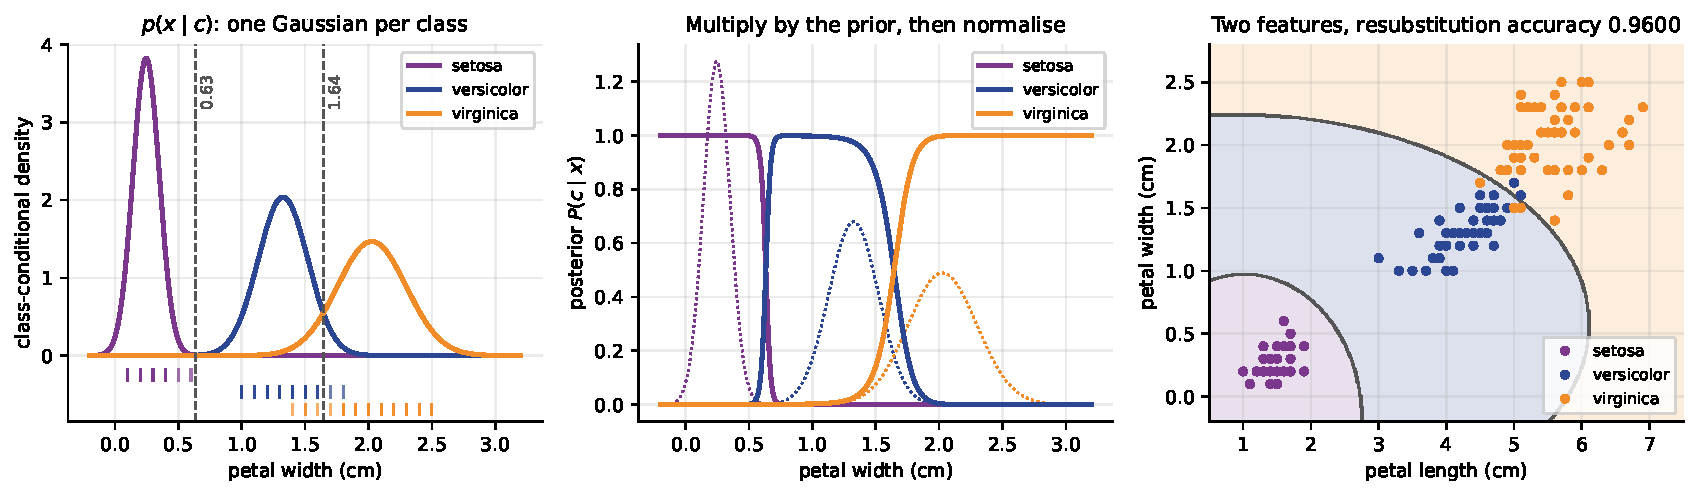
\includegraphics[width=\textwidth]{gaussnb.pdf}
\caption{Left: one fitted Gaussian per class over iris petal width, with the
raw measurements as ticks below and the two decision boundaries dashed.
Centre: the posteriors, obtained by multiplying each density by its prior and
normalising; the dotted curves are the scaled densities. Right: the same
model on two features, resubstitution accuracy $0.9600$.}
\label{fig:gauss}
\end{figure}

\subsection{Measured against harder models}

\begin{lstlisting}
cross_val_score(GaussianNB(), X, y, cv=StratifiedKFold(5, shuffle=True,
                                                       random_state=0)).mean()
\end{lstlisting}
\begin{codeout}
GaussianNB against two others, 5-fold, on four bundled datasets
   dataset           GaussianNB    LogReg  RandForest  fit ms NB  fit ms LR
   iris                  0.9600    0.9600      0.9400       0.45       1.69
   wine                  0.9719    0.9832      0.9719       0.41       1.82
   breast_cancer         0.9385    0.9789      0.9649       0.53       2.40
   digits                0.8508    0.9694      0.9733       1.29     128.02
\end{codeout}

Competitive, not best. It ties logistic regression on \texttt{iris}, matches
the random forest on \texttt{wine}, gives away four points on
\texttt{breast\_cancer} and twelve on \texttt{digits} --- where neighbouring
pixels are strongly dependent, which is precisely what the assumption
forbids.

The last two columns say that fitting is cheap, but do not quote them: they
are milliseconds, and milliseconds belong to a processor rather than to an
algorithm. The reason behind them is exact and does belong on paper.

\begin{codeout}
   dataset            rows x cols  NB passes  LR L-BFGS iterations
   iris                   150 x 4          1                    17
   wine                  178 x 13          1                    15
   breast_cancer         569 x 30          1                    19
   digits               1797 x 64          1                    32
\end{codeout}

\textbf{Naive Bayes makes exactly one pass over the data.} For each column of
each class it accumulates a count, a sum and a sum of squares, divides at the
end, and stops. There is no solver, no step size, no convergence criterion and
nothing that can fail to converge. Logistic regression on the same four
problems needed $15$ to $32$ L-BFGS iterations, each of which is a pass over
every row plus a gradient --- and it does not know in advance how many it will
need. That is where the hundredfold on \texttt{digits} comes from, and unlike
the hundredfold itself, the pass counts are the same on every machine.

\begin{caution}[Do not quote the milliseconds]
The two \texttt{fit ms} columns are the only numbers in these notes that will
not reproduce on your machine, or on this one tomorrow. They depend on the
processor, the BLAS build and what else is running. Quote the pass counts
instead: one against $15$--$32$, and no iteration at all against an iterative
solver. That claim is true everywhere.
\end{caution}

\begin{tryit}
Fit \texttt{GaussianNB()} on all four iris columns and print
\texttt{theta\_.size + var\_.size + len(clf.class\_prior\_) - 1}. You should
get $12 + 12 + 2 = 26$ --- twenty-six numbers is the entire model. Its
five-fold accuracy is $0.9600$ and its resubstitution accuracy is also
$0.9600$: a model with twenty-six parameters and $150$ rows has essentially
nothing to overfit with.
\end{tryit}

% =========================================================================
\section{A good classifier and a bad probability estimator}
\label{sec:calib}

\subsection{The measurement}

Split \texttt{breast\_cancer} $60/40$, fit \texttt{GaussianNB} and a
standardised logistic regression, and compare not just their accuracy but the
quality of the probabilities they emit.

\begin{lstlisting}
from sklearn.metrics import brier_score_loss, log_loss, roc_auc_score
pn = GaussianNB().fit(Xtr, ytr).predict_proba(Xte)[:, 1]
\end{lstlisting}
\begin{codeout}
model                 accuracy     Brier   log loss   ROC AUC
GaussianNB              0.9342    0.0663     1.0444    0.9785
LogisticRegression      0.9649    0.0211     0.0718    0.9965
\end{codeout}

Three points of accuracy behind, but the \textbf{Brier score is three times
worse} and the log loss is fourteen times worse. The Brier score is just the
mean squared error of the predicted probability against the $0/1$ outcome, so
it punishes a confident mistake far harder than accuracy does.

\begin{codeout}
where the predicted probabilities actually sit
   GaussianNB           fraction with max-probability > 0.99 : 0.9649
                        fraction with max-probability > 0.999: 0.9298
                        fraction in [0.1, 0.9]              : 0.0219
                        mean confidence 0.9936 against accuracy 0.9342
   LogisticRegression   fraction with max-probability > 0.99 : 0.7105
                        fraction with max-probability > 0.999: 0.4956
                        fraction in [0.1, 0.9]              : 0.1360
                        mean confidence 0.9626 against accuracy 0.9649
\end{codeout}

\begin{keyidea}
Naive Bayes claims a mean confidence of $\mathbf{0.9936}$ and is right
$\mathbf{0.9342}$ of the time. Logistic regression claims $0.9626$ and is
right $0.9649$ of the time. \textbf{One of these models knows what it does
not know.}
\end{keyidea}

Ninety-three percent of naive Bayes' predictions claim a probability above
$0.999$, and only two percent of them land anywhere between $0.1$ and $0.9$.
It effectively has two outputs.

\subsection{A reliability table}

The direct check: bin the predictions by what they claimed, and look at what
actually happened in each bin.

\begin{codeout}
   GaussianNB
      bin               n    mean p    actual      gap
      [0.00,0.10)      83    0.0014    0.0964  -0.0950
      [0.10,0.30)       3    0.1864    0.0000  +0.1864
      [0.50,0.70)       1    0.5483    1.0000  -0.4517
      [0.70,0.90)       1    0.7451    1.0000  -0.2549
      [0.90,0.99)       1    0.9575    1.0000  -0.0425
      [0.99,1.00)     139    0.9998    0.9496  +0.0501
   LogisticRegression
      bin               n    mean p    actual      gap
      [0.00,0.10)      75    0.0036    0.0000  +0.0036
      [0.10,0.30)       7    0.1967    0.1429  +0.0538
      [0.30,0.50)       5    0.4199    0.8000  -0.3801
      [0.50,0.70)       3    0.5770    0.6667  -0.0896
      [0.70,0.90)      16    0.8547    0.8750  -0.0203
      [0.90,0.99)      29    0.9656    1.0000  -0.0344
      [0.99,1.00)      93    0.9980    1.0000  -0.0020
\end{codeout}

Read the first row of each block. Naive Bayes put $83$ patients in the
bottom bin, claiming an average probability of benign of $0.0014$; nearly
\emph{one in ten of them was benign}. Logistic regression put $75$ patients
in the same bin claiming $0.0036$, and none of them was benign. The two
populated bins of naive Bayes carry gaps of $-0.0950$ and $+0.0501$; the two
populated bins of logistic regression carry $+0.0036$ and $-0.0020$.

\begin{figure}[htbp]
\centering
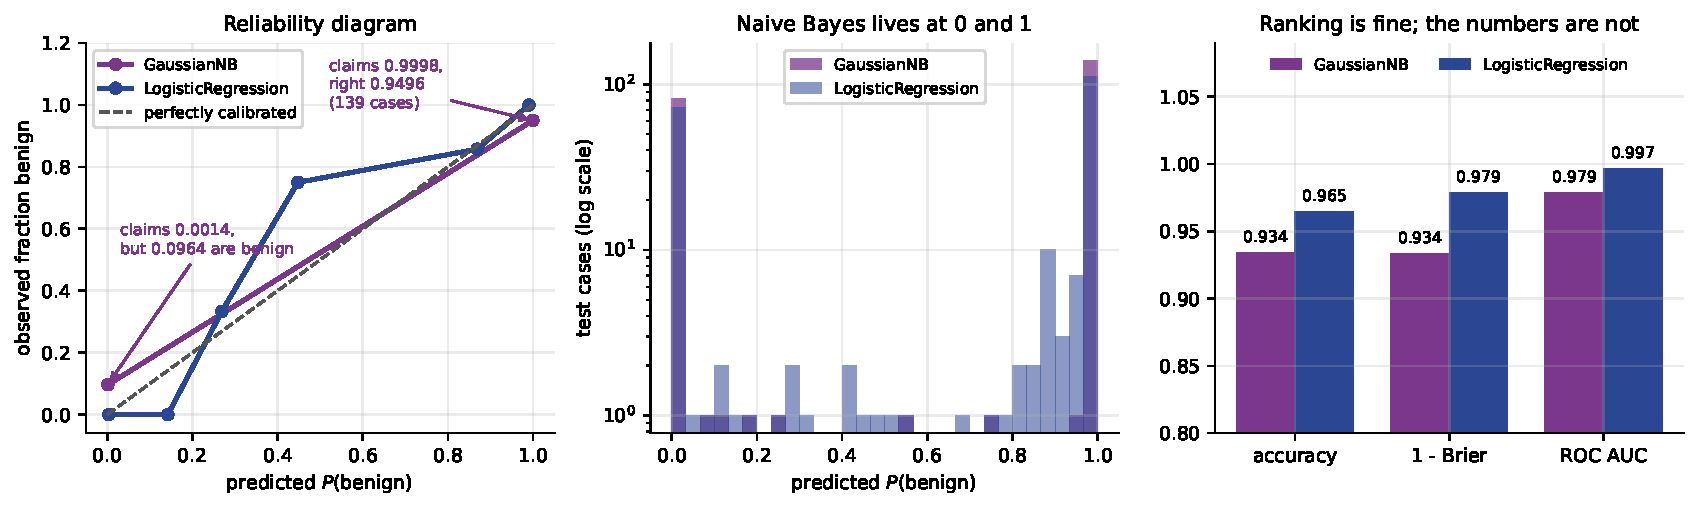
\includegraphics[width=\textwidth]{calibration.pdf}
\caption{Left: the reliability diagram --- a well-calibrated model lies on
the diagonal. Centre: the histogram of predicted probabilities on a
logarithmic count scale; naive Bayes has two bars and almost nothing between
them. Right: the same model scored three ways. Its ROC AUC is $0.979$ against
logistic regression's $0.997$, so the \emph{ranking} is nearly as good --- it
is the numbers that are wrong.}
\label{fig:calib}
\end{figure}

\subsection{Can it be repaired?}

Yes, afterwards, by fitting a second monotone model that maps raw scores to
honest probabilities: a sigmoid (Platt scaling) or a step function
(isotonic regression).

\begin{lstlisting}
from sklearn.calibration import CalibratedClassifierCV
cal = CalibratedClassifierCV(GaussianNB(), method="sigmoid", cv=5).fit(Xtr, ytr)
\end{lstlisting}
\begin{codeout}
calibrating it afterwards repairs the probabilities
   model                               accuracy    Brier      AUC
   GaussianNB, raw                       0.9342   0.0663   0.9785
   GaussianNB + sigmoid                  0.9342   0.0626   0.9751
   GaussianNB + isotonic                 0.9211   0.0567   0.9646
   both cut the Brier score. Report the AUC honestly: neither improves
   it, because CalibratedClassifierCV averages five fold-models each
   fitted on 80% of only 341 rows, and isotonic also reorders ties.
   The lesson is the Brier column: calibration repairs the NUMBERS.
\end{codeout}

The Brier score improves both times, from $0.0663$ to $0.0626$ and $0.0567$.
The AUC does not, and it is worth being clear why rather than pretending:
\texttt{CalibratedClassifierCV} refits the base estimator on five internal
folds of only $341$ training rows and averages the results, and isotonic
regression is free to reorder tied scores. On a larger training set the
ranking loss disappears; here it does not.

\begin{caution}[The practical rule]
Use \texttt{predict} freely --- naive Bayes ranks well. Treat
\texttt{predict\_proba} with suspicion. \textbf{Calibrate before you use a
naive Bayes probability to make a decision that has a cost attached}, such
as a threshold on a medical or a credit decision. The scikit-learn user
guide says the same thing in one sentence: ``although naive Bayes is known
as a decent classifier, it is known to be a bad estimator''.
\end{caution}

% =========================================================================
\section{Where the independence assumption genuinely hurts}
\label{sec:hurts}

The previous section measured the symptom. This one is the mechanism, and
there are three separate failure modes worth telling apart.

\subsection{Redundant features: counting the same evidence twice}

Start with four genuinely independent informative features and add $k$
near-copies of the first one. The copies carry no new information at all.

\begin{codeout}
A. duplicate one informative feature k times
   4 independent informative features, class separation 1.6 sd
    copies of f0    d  GaussianNB    LogReg  RandForest
               0    4      0.9475    0.9467      0.9367
               1    5      0.9350    0.9483      0.9350
               3    7      0.9083    0.9467      0.9283
               7   11      0.8633    0.9458      0.9267
              15   19      0.8367    0.9467      0.9233
              31   35      0.8200    0.9483      0.9133
   GaussianNB lost 0.1275 of accuracy; logistic regression lost -0.0017
\end{codeout}

\begin{keyidea}
Naive Bayes fell from $0.9475$ to $0.8200$ on \emph{no new information},
because the product rule treats every factor as an independent observation.
Thirty-two copies of one measurement are counted as thirty-two pieces of
evidence. Logistic regression fits the columns jointly, splits the weight
between them, and does not move at all --- it ends $0.0017$
\emph{higher} than it started, which is noise, not improvement.
\end{keyidea}

And the confidence moves the wrong way while this happens:

\begin{codeout}
   and what it does to the confidence
      k= 0  mean confidence 0.9457   accuracy 0.9556   fraction > 0.999 0.2833   Brier 0.0331
      k=31  mean confidence 0.9916   accuracy 0.8139   fraction > 0.999 0.9139   Brier 0.1802
\end{codeout}

Confidence rises from $0.9457$ to $0.9916$ while accuracy falls from $0.9556$
to $0.8139$, and the Brier score gets more than five times worse. The
proportion of predictions made with confidence above $0.999$ goes from about
a quarter to more than nine tenths. \textbf{This
is exactly the mechanism behind Section~\ref{sec:calib}}: inflating the
log-odds by double-counting pushes the sigmoid into saturation, so the
posteriors pile up at $0$ and $1$.

\subsection{On real data}

\texttt{breast\_cancer} is not an artificial example of this. Its thirty
columns are ten cell measurements recorded three ways each --- a mean, a
standard error and a ``worst'' value.

\begin{codeout}
   mean |correlation| between the 30 columns: 0.3949
   pairs with |r| > 0.9: 21 of 435
   feature set                          d  GaussianNB    LogReg
   all 30                              30      0.9385    0.9789
   the 10 'mean' columns               10      0.9104    0.9455
   the 10 'worst' columns              10      0.9456    0.9789
   mean + worst (20)                   20      0.9420    0.9789
\end{codeout}

Ten columns beat thirty: the \texttt{worst} block alone gives
\texttt{GaussianNB} $0.9456$ against $0.9385$ for all thirty. Discarding
two-thirds of the data improved the model, and logistic regression --- which
scores $0.9789$ on both --- was indifferent.

\begin{figure}[htbp]
\centering
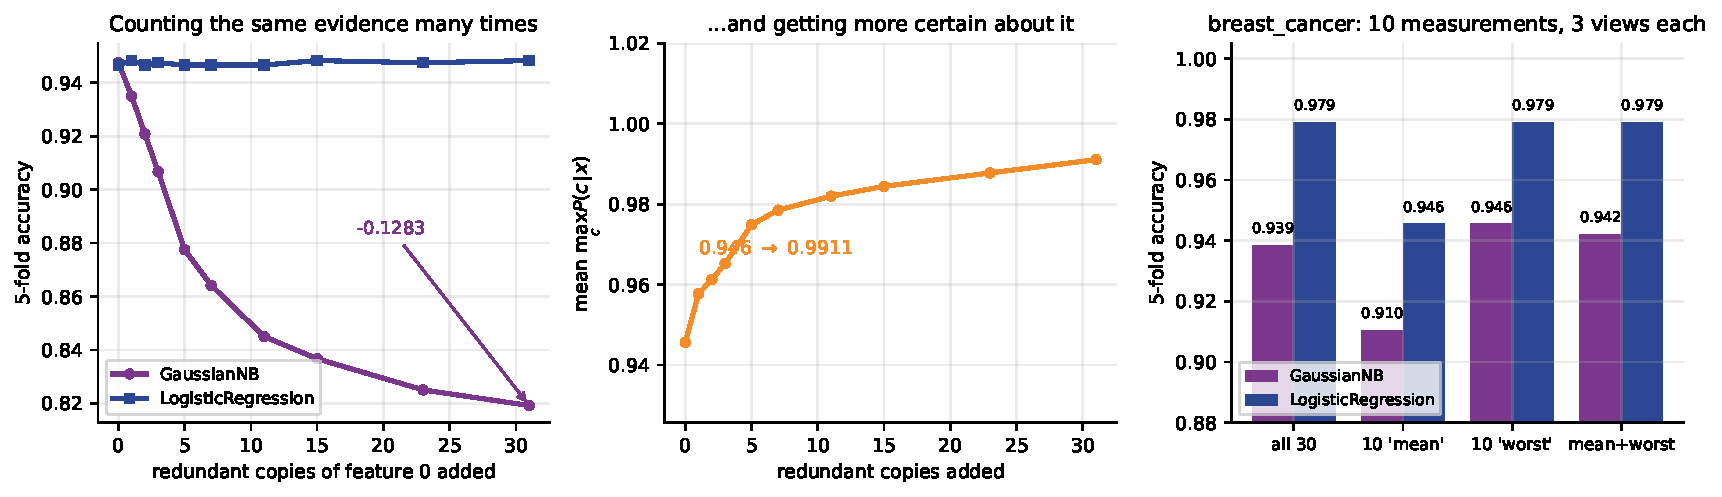
\includegraphics[width=\textwidth]{correlated.pdf}
\caption{Left: five-fold accuracy against the number of redundant copies
added. Centre: mean $\max_c P(c \mid x)$ over the same sweep, rising from
$0.9457$ to $0.9911$ as accuracy falls. Right: the real
\texttt{breast\_cancer} feature blocks --- naive Bayes in purple is helped by
dropping columns, logistic regression in blue is not.}
\label{fig:corr}
\end{figure}

\begin{keyidea}
For naive Bayes, \textbf{removing correlated columns is a modelling step,
not tidying}. It is the one place where feature selection reliably pays for
this algorithm. Rules of thumb: keep one column from each block of strongly
correlated measurements, or reduce with PCA, whose components are
uncorrelated by construction.
\end{keyidea}

\subsection{Interactions: XOR, which no factorised model can learn}

A different failure, and worth keeping separate in your head. Two binary
features with a little noise, and the label is their exclusive-or.

The four $(u,v)$ cells are built in equal numbers rather than drawn at
random, so the design is exactly symmetric and the result cannot depend on a
lucky sample: each feature is uninformative \emph{by construction}. Only the
noise and the row order come from the seed.

\begin{codeout}
C. the XOR problem
   1200 rows, 300 in each of the four (u,v) cells by construction
   GaussianNB   0.4600
   LogReg       0.4600
   RandForest   0.9833
      class 0: mean u 0.5063  mean v 0.4974  corr(u,v|y) +0.8621
      class 1: mean u 0.4819  mean v 0.4936  corr(u,v|y) -0.8573
\end{codeout}

Chance level, on a perfectly learnable problem --- both models land a shade
\emph{below} $0.5$, which is what a cross-validated estimate of a coin flip
looks like. Read the last two lines. Within each class the means of $u$ and
$v$ are both about $0.5$, so \emph{each feature alone is completely
uninformative}: every factor $P(x_j \mid c)$ is essentially identical for
both classes and their product cannot separate them. All the signal is in the
\emph{correlation}, which is $+0.86$ in one class and $-0.86$ in the other ---
exactly the quantity the naive assumption discards. A random forest, which can
represent interactions, gets $0.9833$.

\subsection{So why does anyone use it? The Domingos and Pazzani answer}

Fit the same models on a shrinking training set, averaged over thirty random
splits.

\begin{codeout}
D. NB can win even when the probabilities are wrong
    n train  GaussianNB    LogReg  RandForest
         20      0.9271    0.9276      0.9161
         40      0.9366    0.9502      0.9287
         80      0.9374    0.9640      0.9393
        200      0.9357    0.9711      0.9478
        400      0.9385    0.9763      0.9548
\end{codeout}

At $n = 20$ --- twenty patients, thirty features --- naive Bayes is level
with logistic regression and ahead of the random forest. It estimates
$30 \times 2$ means and $30 \times 2$ variances, each from ten rows, and has
almost no variance to bleed because it never fits a joint anything. By
$n = 400$ logistic regression is four points ahead, but you frequently do not
have $400$ rows.

\begin{keyidea}
Domingos and Pazzani's result in one sentence: \textbf{a wrong probability
model can still put the right class on top}, because the argmax depends only
on the ordering of the scores, not on their values. Naive Bayes is biased and
almost unbiased-variance-free, and on small or wide data that is the better
end of the trade.
\end{keyidea}

\subsection{The complete failure list}

\begin{center}\small
\begin{tabular}{@{}p{3.5cm}p{4.3cm}p{6.2cm}@{}}
\toprule
\textbf{Failure} & \textbf{Symptom} & \textbf{Fix}\\
\midrule
zero frequency & a posterior of exactly $0$ or $1$ &
  Laplace smoothing, $\alpha \ge$ a small positive number\\
underflow & accuracy collapses on long documents &
  work in logs; use the library, which already does\\
redundant features & confidence rises as accuracy falls &
  drop correlated columns, or use PCA\\
interactions & chance-level accuracy on a learnable problem &
  a tree, a forest or a kernel method\\
badly calibrated output & \texttt{predict\_proba} is always
  $\approx 0$ or $\approx 1$ &
  \texttt{CalibratedClassifierCV}; or use only the ranking\\
continuous but non-Gaussian & \texttt{GaussianNB} underperforms &
  discretise into bins and use \texttt{CategoricalNB}, or transform the
  feature\\
$\alpha$ left at the default & a point or two of accuracy on text &
  cross-validate $\alpha$\\
negative values in \texttt{MultinomialNB} & a \texttt{ValueError} &
  \texttt{MultinomialNB} requires non-negative counts; do not standardise
  text features\\
\bottomrule
\end{tabular}
\end{center}

% =========================================================================
\section{Summary}
\label{sec:summary}

\begin{enumerate}[leftmargin=*]
  \item Bayes' theorem is the product rule written twice and divided:
    $P(c \mid x) = P(x \mid c)P(c)/P(x)$, with the four names
    \textbf{posterior}, \textbf{likelihood}, \textbf{prior},
    \textbf{evidence}. It is a rearrangement, not an assumption.
  \item The medical test --- prevalence $1\%$, sensitivity $99\%$,
    specificity $95\%$ --- gives $P(D \mid +) = 99/594 = 1/6 =
    \mathbf{0.166667}$. Confusing this with the sensitivity is the
    \textbf{base-rate fallacy}.
  \item In natural frequencies: of $10{,}000$ people, $594$ test positive and
    $99$ are ill. False positives outnumber true positives \emph{five to
    one}. Two million simulated people give $0.165611$.
  \item Specificity is the lever, not sensitivity: $95\% \to 99.9\%$ takes
    the posterior from $0.1667$ to $0.9091$. Raising prevalence to $20\%$
    takes it to $0.8319$.
  \item Evidence can be absorbed all at once or one piece at a time:
    $P(D \mid +,+) = 0.798387$ either way. \textbf{Yesterday's posterior is
    today's prior.}
  \item \textbf{ML} maximises $P(x \mid c)$; \textbf{MAP} maximises
    $P(x \mid c)P(c)$. Here they disagree, because a likelihood ratio of
    $19.8$ cannot overcome prior odds of $99$. Posterior odds $=$ likelihood
    ratio $\times$ prior odds.
  \item The full joint likelihood needs $C(2^d - 1)$ parameters: at $d = 30$,
    $2{,}147{,}483{,}646$ against $569$ rows. It exceeds the available data at
    $\mathbf{d = 9}$.
  \item \textbf{The naive assumption}: $P(x_1,\ldots,x_d \mid c) =
    \prod_j P(x_j \mid c)$, independence \emph{given the class}. On the
    tennis table that is $70$ free parameters down to $\mathbf{12}$, and
    $0.194$ rows per joint cell up to at least five rows per estimate.
  \item Worked by hand on $(\text{Sunny},\text{Cool},\text{High},
    \text{Strong})$: $\text{score}(\text{No}) = 0.02057143$,
    $\text{score}(\text{Yes}) = 0.00529101$, evidence $0.02586243$,
    $P(\text{No} \mid x) = \mathbf{0.795417}$ ---
    and \texttt{CategoricalNB} agrees to $7.68 \times 10^{-12}$.
  \item \textbf{Zero frequency}: $P(\text{Overcast} \mid \text{No}) = 0/5$
    makes the whole product zero and the class impossible. Laplace,
    $(0+1)/(5+3) = 0.125$, turns $P(\text{No} \mid x)$ from $0.000000$ into
    $\mathbf{0.278417}$. Add $\alpha$ on top and $\alpha n_j$ below, where
    $n_j$ is the number of \emph{levels}.
  \item Twelve of the $36$ possible days contain a zero; on this table the
    label never flips (mean posterior change $0.0942$, maximum $0.4356$).
    On the ten-row table of question~3 it does flip. As
    $\alpha \to \infty$ the posterior tends to the prior $9/14 = 0.6429$.
  \item \textbf{Text.} $P(w \mid c) = (T_{cw}+\alpha)/(\sum T_{cw'} + \alpha
    V)$. On the twelve-message corpus only $5$ of $51$ words appear in both
    classes; ``click the free link'' scores $\log$ spam $-12.887198$ against
    ham $-16.973632$, so $P(\text{spam}) = 0.983479$.
  \item \textbf{Underflow.} A product of per-token probabilities becomes
    exactly $0.0$ at $\mathbf{148}$ tokens. Multiplying instead of summing
    logs took accuracy from $0.9722$ to $\mathbf{0.5056}$, silently. Recover a
    posterior with log-sum-exp: $a_{\max} + \log\sum e^{a - a_{\max}}$.
  \item \textbf{Gaussian naive Bayes} stores one mean and one variance per
    feature per class. Iris petal width $1.7$\,cm gives
    $P(\text{virginica} \mid x) = 0.685166$; boundaries at $0.6333$ and
    $1.6437$\,cm; twenty-six parameters for the whole four-feature model. It
    fits \texttt{digits} in \emph{one} pass over the data against logistic
    regression's $32$ L-BFGS iterations.
  \item \textbf{Good classifier, bad probability estimator}: mean confidence
    $\mathbf{0.9936}$ against accuracy $\mathbf{0.9342}$, $93\%$ of
    predictions above $0.999$, Brier $0.0663$ against $0.0211$ --- but AUC
    $0.9785$ against $0.9965$. The ranking is fine; the numbers are not.
  \item \textbf{Redundant features are the mechanism.} Thirty-one copies of
    one column took accuracy $0.9475 \to 0.8200$ and confidence
    $0.9457 \to 0.9916$. On \texttt{breast\_cancer}, the ten
    \texttt{worst} columns ($0.9456$) beat all thirty ($0.9385$).
  \item \textbf{Interactions are a different failure.} On XOR naive Bayes
    scores $0.4600$ while a random forest scores $0.9833$, because each
    feature alone is uninformative and all the signal is in the
    within-class correlation.
  \item It survives because at $n = 20$ it ties logistic regression
    ($0.9271$ against $0.9276$): almost no parameters, so almost no variance.
    \textbf{A wrong probability model can still put the right class on
    top.}
\end{enumerate}

% =========================================================================
\section{Practice questions}
\label{sec:practice}

Attempt them before reading Section~\ref{sec:solutions}. Questions 1, 2, 3, 5
and 7 are of the type the class test asks; do those with a pen, not a laptop.

\begin{enumerate}[leftmargin=*, itemsep=0.55em]

\item \textbf{(Base rates by hand.)} A different disease has a prevalence of
  $2\%$. A test for it has sensitivity $90\%$ and specificity $90\%$.
  \begin{enumerate}[label=(\alph*)]
    \item Compute $P(D \mid +)$ from the formula, showing the two joint
      probabilities and the evidence.
    \item Reproduce the answer with a natural-frequency table over
      $10{,}000$ people.
    \item Compute $P(D \mid -)$.
    \item What specificity would the test need, at the same prevalence and
      sensitivity, for a positive result to mean a $50\%$ chance of disease?
  \end{enumerate}

\item \textbf{(Sequential updating by hand.)} The patient of question~1
  tests positive, and then takes the same test again independently.
  \begin{enumerate}[label=(\alph*)]
    \item Compute $P(D \mid +,+)$ directly.
    \item Compute it again by treating your answer to question~1(a) as the
      prior for a second single update, and confirm you get the same number.
    \item Now suppose the second test is \emph{negative}. Compute
      $P(D \mid +,-)$, and explain the answer using the likelihood ratios
      $\text{LR}^{+} = P(+ \mid D)/P(+ \mid \lnot D)$ and
      $\text{LR}^{-} = P(- \mid D)/P(- \mid \lnot D)$.
  \end{enumerate}

\item \textbf{(Naive Bayes by hand, with and without smoothing.)} Ten
  customers, three categorical features, and whether they bought.

  \begin{center}\small
  \begin{tabular}{@{}rlllc@{}}
  \toprule
  \# & Age & Income & Student & \textbf{Buys}\\
  \midrule
  1 & Young & High & No & No\\
  2 & Young & High & Yes & No\\
  3 & Middle & High & No & Yes\\
  4 & Old & Medium & No & Yes\\
  5 & Old & Low & Yes & Yes\\
  6 & Old & Low & Yes & No\\
  7 & Middle & Low & Yes & Yes\\
  8 & Young & Medium & No & No\\
  9 & Young & Low & Yes & Yes\\
  10 & Old & Medium & Yes & Yes\\
  \bottomrule
  \end{tabular}
  \end{center}

  \begin{enumerate}[label=(\alph*)]
    \item Give the priors and the full conditional probability tables.
    \item Classify $x = (\text{Young}, \text{Low}, \text{Yes})$ with
      $\alpha = 0$. Give both unnormalised scores and both posteriors to six
      decimal places.
    \item Repeat with Laplace smoothing, $\alpha = 1$. State the level count
      you used in each denominator. What happens to the prediction?
    \item Classify $x = (\text{Middle}, \text{High}, \text{No})$ with
      $\alpha = 0$ and explain the posterior you get in one sentence.
  \end{enumerate}

\item \textbf{(Counting parameters.)} A dataset has four categorical features
  with $4$, $3$, $3$ and $2$ levels, and three classes.
  \begin{enumerate}[label=(\alph*)]
    \item How many cells does the full class-conditional joint table have,
      and how many \emph{free} parameters?
    \item How many free parameters does naive Bayes need for the same
      features?
    \item Repeat both counts for $12$ binary features and two classes.
    \item In one sentence, why is the naive count linear in $d$ while the
      joint count is exponential?
  \end{enumerate}

\item \textbf{(Text naive Bayes and the zero-frequency problem.)} A corpus of
  six messages, three spam and three ham.

  \begin{center}\small
  \begin{tabular}{@{}ll@{}}
  \toprule
  \textbf{spam} & \textbf{ham}\\
  \midrule
  buy cheap pills now & meeting at noon today\\
  cheap loan offer now & project report due today\\
  buy now limited offer & see you at the meeting\\
  \bottomrule
  \end{tabular}
  \end{center}

  The vocabulary has $17$ distinct words; spam contains $12$ tokens in total
  and ham $13$. Classify \texttt{"cheap offer today"} with equal priors.
  \begin{enumerate}[label=(\alph*)]
    \item First with $\alpha = 0$. What happens, and why?
    \item Then with Laplace $\alpha = 1$. Give $P(w \mid S)$ and
      $P(w \mid H)$ for all three words, the two log scores, and
      $P(\text{spam} \mid \text{message})$.
  \end{enumerate}

\item \textbf{(Underflow.)} A naive Bayes model assigns every word in a
  document a conditional probability of about $0.002$.
  \begin{enumerate}[label=(\alph*)]
    \item Estimate, using logarithms base $10$, the order of magnitude of the
      product for a $200$-word document.
    \item The smallest positive \texttt{float64} is about
      $4.9 \times 10^{-324}$. At roughly how many words does the product
      underflow to exactly $0.0$?
    \item What does the sum of natural logarithms evaluate to at $200$ words?
    \item A classmate says ``it does not matter, both classes underflow
      together so the comparison still works''. Correct them, quoting a
      measurement from these notes.
  \end{enumerate}

\item \textbf{(Gaussian naive Bayes by hand, and ML against MAP.)} A single
  continuous feature. Class $0$ has $\mu_0 = 5.0$, $\sigma_0 = 1.0$ and prior
  $0.6$; class $1$ has $\mu_1 = 6.5$, $\sigma_1 = 1.5$ and prior $0.4$. An
  instance arrives with $x = 6.0$.
  \begin{enumerate}[label=(\alph*)]
    \item Compute both class-conditional densities to six decimal places.
    \item Give the ML prediction and the MAP prediction. Do they agree?
    \item Give the posterior probabilities.
    \item Why is it acceptable for a ``probability'' here to be larger than
      $1$ in some other example?
  \end{enumerate}

\item \textbf{(Reading a confidence report.)} A colleague reports that their
  \texttt{GaussianNB} model on a medical dataset has accuracy $0.93$ and that
  ``$95\%$ of its predictions come with probability above $0.99$, so we can
  automate those and only send the rest for review''.
  \begin{enumerate}[label=(\alph*)]
    \item What is wrong with the plan?
    \item Describe the single measurement you would run to demonstrate it,
      and what you would expect to see.
    \item What would you do instead?
  \end{enumerate}

\item \textbf{(Debugging.)} A classmate writes:

\begin{lstlisting}
enc = OrdinalEncoder()
Xe  = enc.fit_transform(df[["outlook","temp","humidity","wind"]])
nb  = CategoricalNB(alpha=0.0, force_alpha=True).fit(Xe, y)
p   = nb.predict_proba(enc.transform(new_rows))
print("confidence", p.max(axis=1).mean())     # prints 1.0
\end{lstlisting}

  and reports ``the model is $100\%$ confident on every new record''.
  Identify three separate problems and give the corrected code.

\item \textbf{(Correlated features.)} A colleague has a table of gene
  expression with $60$ patients and $4000$ measurements, many of them
  strongly correlated because the genes lie in the same pathways. They plan
  to use \texttt{GaussianNB} and report \texttt{predict\_proba} to a
  clinician.
  \begin{enumerate}[label=(\alph*)]
    \item Predict what will happen to the accuracy and to the confidence,
      quoting the relevant measurements from these notes.
    \item Would you expect naive Bayes to beat logistic regression at
      $n = 60$? Quote a number.
    \item Give three concrete changes to the plan.
  \end{enumerate}

\end{enumerate}

% =========================================================================
\section{Solutions}
\label{sec:solutions}

\begin{enumerate}[leftmargin=*, itemsep=0.7em]

\item
  \begin{enumerate}[label=(\alph*)]
    \item $P(+, D) = 0.90 \times 0.02 = \mathbf{0.0180}$ and
      $P(+, \lnot D) = 0.10 \times 0.98 = \mathbf{0.0980}$, so the evidence
      is $P(+) = 0.0180 + 0.0980 = \mathbf{0.1160}$ and
      \[
        P(D \mid +) = \frac{0.0180}{0.1160} = \mathbf{0.155172}.
      \]
    \item Of $10{,}000$ people, $200$ have the disease and $180$ of those
      test positive; $9800$ do not and $980$ of those test positive. Total
      positives $180 + 980 = 1160$, of whom $180$ are ill:
      $180/1160 = \mathbf{0.155172}$.

      \begin{center}\small
      \begin{tabular}{@{}lrrr@{}}
      \toprule
       & test $+$ & test $-$ & total\\
      \midrule
      disease & \textbf{180} & 20 & 200\\
      healthy & \textbf{980} & 8820 & 9800\\
      \midrule
      total & \textbf{1160} & 8840 & 10000\\
      \bottomrule
      \end{tabular}
      \end{center}
    \item $P(D \mid -) = \dfrac{0.10 \times 0.02}
      {0.10 \times 0.02 + 0.90 \times 0.98}
      = \dfrac{0.002}{0.884} = \mathbf{0.002262}$. A negative result is
      informative: it takes you from $2\%$ to $0.23\%$.
    \item Set $0.90 \times 0.02 = (1 - s)(0.98)$, so
      $1 - s = 0.018/0.98 = 0.018367$ and
      $s = \mathbf{0.981633}$. The test would need to be $98.16\%$ specific
      merely to make a positive an even-money bet.
  \end{enumerate}

\item
  \begin{enumerate}[label=(\alph*)]
    \item $P(D \mid +,+) = \dfrac{0.90^2 \times 0.02}
      {0.90^2 \times 0.02 + 0.10^2 \times 0.98}
      = \dfrac{0.0162}{0.0162 + 0.0098} = \dfrac{0.0162}{0.0260}
      = \mathbf{0.623077}$.
    \item Take the prior to be $0.155172$ from question~1(a):
      \[
        \frac{0.90 \times 0.155172}
             {0.90 \times 0.155172 + 0.10 \times 0.844828}
        = \frac{0.139655}{0.139655 + 0.084483}
        = \mathbf{0.623077}.
      \]
      The same number, which is the point: Bayes' theorem is an updating
      rule, and evidence may be absorbed in any order or all at once.
    \item Starting again from $0.155172$ and observing a negative:
      \[
        P(D \mid +,-) = \frac{0.10 \times 0.155172}
          {0.10 \times 0.155172 + 0.90 \times 0.844828}
        = \frac{0.015517}{0.775862} = \mathbf{0.020000}.
      \]
      \textbf{Exactly the prior.} Here $\text{LR}^{+} = 0.90/0.10 = 9$ and
      $\text{LR}^{-} = 0.10/0.90 = 1/9$, and $9 \times 1/9 = 1$. In odds
      form the two observations multiply the prior odds by $1$, so they
      cancel completely. This happens whenever sensitivity and specificity
      are equal.
  \end{enumerate}

\item
  \begin{enumerate}[label=(\alph*)]
    \item Six \emph{Yes} and four \emph{No}, so
      $P(\text{Yes}) = 6/10 = 0.6$ and $P(\text{No}) = 4/10 = 0.4$.

      \begin{center}\small
      \begin{tabular}{@{}llcc@{}}
      \toprule
      Feature & Level & given Yes ($N=6$) & given No ($N=4$)\\
      \midrule
      Age & Middle & 2/6 & \textbf{0/4}\\
          & Old    & 3/6 & 1/4\\
          & Young  & 1/6 & 3/4\\
      \midrule
      Income & High   & 1/6 & 2/4\\
             & Low    & 3/6 & 1/4\\
             & Medium & 2/6 & 1/4\\
      \midrule
      Student & No  & 2/6 & 2/4\\
              & Yes & 4/6 & 2/4\\
      \bottomrule
      \end{tabular}
      \end{center}
    \item With $\alpha = 0$:
      \begin{align*}
        \text{score}(\text{No})
          &= \tfrac{4}{10}\cdot\tfrac{3}{4}\cdot\tfrac{1}{4}
             \cdot\tfrac{2}{4} = \mathbf{0.03750000}\\
        \text{score}(\text{Yes})
          &= \tfrac{6}{10}\cdot\tfrac{1}{6}\cdot\tfrac{3}{6}
             \cdot\tfrac{4}{6} = \mathbf{0.03333333}
      \end{align*}
      Evidence $= 0.07083333$, so $P(\text{No} \mid x) = \mathbf{0.529412}$
      and $P(\text{Yes} \mid x) = \mathbf{0.470588}$. \textbf{Prediction:
      No.}
    \item Age has $3$ levels, Income has $3$, Student has $2$. So the
      \emph{No} denominators are $4+3 = 7$, $4+3 = 7$ and $4+2 = 6$, and the
      \emph{Yes} denominators are $6+3 = 9$, $6+3 = 9$ and $6+2 = 8$.
      \begin{align*}
        \text{score}(\text{No})
          &= \tfrac{4}{10}\cdot\tfrac{3+1}{7}\cdot\tfrac{1+1}{7}
             \cdot\tfrac{2+1}{6} = \mathbf{0.03265306}\\
        \text{score}(\text{Yes})
          &= \tfrac{6}{10}\cdot\tfrac{1+1}{9}\cdot\tfrac{3+1}{9}
             \cdot\tfrac{4+1}{8} = \mathbf{0.03703704}
      \end{align*}
      Evidence $= 0.06969010$, so $P(\text{Yes} \mid x) = \mathbf{0.531453}$
      and $P(\text{No} \mid x) = \mathbf{0.468547}$. \textbf{The prediction
      flips to Yes.} Smoothing is not always cosmetic: here it changes the
      label, because the two scores were nearly equal and the smoothing
      pulls the minority class's small counts towards uniformity more than
      the majority class's.

      Verified: \texttt{CategoricalNB(alpha=1e-10)} returns
      \texttt{No 0.529412 Yes 0.470588} and
      \texttt{CategoricalNB(alpha=1.0)} returns
      \texttt{No 0.468547 Yes 0.531453}.
    \item $\text{Middle}$ never occurs with $\text{No}$, so
      $P(\text{Middle} \mid \text{No}) = 0/4 = 0$ and
      $\text{score}(\text{No}) = \tfrac{4}{10}\cdot 0 \cdot
      \tfrac{2}{4}\cdot\tfrac{2}{4} = 0$ exactly, while
      $\text{score}(\text{Yes}) = \tfrac{6}{10}\cdot\tfrac{2}{6}
      \cdot\tfrac{1}{6}\cdot\tfrac{2}{6} = 0.01111111$. So
      $P(\text{Yes} \mid x) = \mathbf{1.000000}$ --- \textbf{the model
      declares ``No'' impossible on the evidence of four rows}, which is why
      $\alpha > 0$ is the default. With $\alpha = 1$ the same instance gives
      $P(\text{Yes} \mid x) = 0.576471$.
  \end{enumerate}

\item
  \begin{enumerate}[label=(\alph*)]
    \item $4 \times 3 \times 3 \times 2 = \mathbf{72}$ cells per class. Each
      class's table must sum to $1$, so it has $71$ free parameters, and with
      three classes that is $3 \times 71 = \mathbf{213}$.
    \item $(4-1) + (3-1) + (3-1) + (2-1) = 8$ per class, so
      $3 \times 8 = \mathbf{24}$, plus $2$ free parameters for the priors.
    \item Joint: $2 \times (2^{12} - 1) = \mathbf{8190}$. Naive:
      $2 \times 12 = \mathbf{24}$. \emph{Note the coincidence: $24$ in both
      parts (b) and (c). The joint counts, $213$ and $8190$, are not close at
      all.}
    \item Because the naive model stores one distribution \emph{per feature}
      and the number of features grows linearly, whereas the joint model
      stores one number \emph{per combination of feature values} and the
      number of combinations is a product.
  \end{enumerate}

\item
  \begin{enumerate}[label=(\alph*)]
    \item With $\alpha = 0$, \emph{today} never appears in spam so
      $P(\text{today} \mid S) = 0$, and \emph{cheap} and \emph{offer} never
      appear in ham so $P(\text{cheap} \mid H) = P(\text{offer} \mid H) = 0$.
      \textbf{Both class scores are exactly $0.000000$.} The model has no
      opinion at all, and the argmax is decided by array order rather than by
      evidence.
    \item With $\alpha = 1$, $V = 17$, spam tokens $12$, ham tokens $13$:

      \begin{center}\small
      \begin{tabular}{@{}lcccc@{}}
      \toprule
      word & $n(S)$ & $n(H)$ & $P(w \mid S)$ & $P(w \mid H)$\\
      \midrule
      cheap & 2 & 0 & $(2{+}1)/(12{+}17) = 0.103448$ &
        $(0{+}1)/(13{+}17) = 0.033333$\\
      offer & 2 & 0 & $0.103448$ & $0.033333$\\
      today & 0 & 2 & $(0{+}1)/29 = 0.034483$ & $(2{+}1)/30 = 0.100000$\\
      \bottomrule
      \end{tabular}
      \end{center}

      Log scores, starting from $\log 0.5 = -0.693147$ for each class:
      \[
        \text{spam} = \mathbf{-8.597810}, \qquad
        \text{ham}  = \mathbf{-9.798127}, \qquad
        \text{margin} = 1.200317 .
      \]
      \[
        P(\text{spam} \mid \text{message})
          = \frac{1}{1 + e^{-1.200317}} = \mathbf{0.768581}.
      \]
      \texttt{MultinomialNB(alpha=1)} returns $0.768581$. Note how much less
      confident this is than the earlier example: one strong ham word against
      two strong spam words is a real contest, and the model says so.
  \end{enumerate}

\item
  \begin{enumerate}[label=(\alph*)]
    \item $\log_{10} 0.002 = -2.699$, so $200$ words give
      $200 \times (-2.699) = -539.8$, that is a product of order
      $\mathbf{10^{-540}}$.
    \item Solve $0.002^{k} = 4.9 \times 10^{-324}$:
      $k = -323.3 / -2.699 \approx 120$. Running it, the product first
      becomes exactly $0.0$ at $\mathbf{k = 120}$. So a document of about
      $120$ words is already too long.
    \item $200 \times \ln 0.002 = 200 \times (-6.214608) =
      \mathbf{-1242.9216}$ --- a perfectly ordinary floating-point number.
    \item They are wrong twice over. First, the classes do \emph{not}
      necessarily underflow together: on the measured run, at $240$ tokens
      all $180$ documents had \emph{both} scores at $0.0$, and the comparison
      \texttt{0.0 > 0.0} evaluates to \texttt{False}, so every document is
      assigned to whichever class the code happens to check second.
      Accuracy fell from $\mathbf{0.9722}$ to $\mathbf{0.5056}$ with no error
      raised. Second, even when only one class underflows the surviving
      comparison is between a denormalised number that has lost most of its
      precision and zero, which is not a reliable ranking.
  \end{enumerate}

\item
  \begin{enumerate}[label=(\alph*)]
    \item
      \[
        p(6.0 \mid c_0) = \frac{1}{1.0\sqrt{2\pi}}
          e^{-\frac{(6.0-5.0)^2}{2 \times 1.0^2}}
          = 0.398942 \times e^{-0.5} = \mathbf{0.241971}
      \]
      \[
        p(6.0 \mid c_1) = \frac{1}{1.5\sqrt{2\pi}}
          e^{-\frac{(6.0-6.5)^2}{2 \times 1.5^2}}
          = 0.265962 \times e^{-0.111111} = \mathbf{0.251589}
      \]
    \item \textbf{ML picks class $1$}, because $0.251589 > 0.241971$.
      \textbf{MAP picks class $0$}, because
      $0.241971 \times 0.6 = \mathbf{0.145182}$ beats
      $0.251589 \times 0.4 = \mathbf{0.100636}$. \textbf{They disagree}: the
      instance is very slightly better explained by class $1$, but class $0$
      is half again as common, and the prior wins.
    \item $P(c_0 \mid x) = 0.145182 / (0.145182 + 0.100636) =
      \mathbf{0.590610}$ and $P(c_1 \mid x) = \mathbf{0.409390}$.
    \item Because $p(x \mid c)$ is a probability \emph{density}, not a
      probability. A density integrates to $1$ over its whole range but may
      take any non-negative value at a point; a narrow Gaussian has a tall
      peak. Only after multiplying by the priors and dividing by the evidence
      do you get numbers that must lie in $[0,1]$.
  \end{enumerate}

\item
  \begin{enumerate}[label=(\alph*)]
    \item The plan assumes that ``probability above $0.99$'' means ``wrong
      about one time in a hundred''. For naive Bayes it does not.
      \texttt{GaussianNB} on \texttt{breast\_cancer} produced a mean
      confidence of $0.9936$ against an accuracy of $0.9342$; $93\%$ of its
      predictions claimed better than $0.999$ and only $2.2\%$ landed between
      $0.1$ and $0.9$. The threshold selects almost the whole dataset and
      therefore selects almost all the errors with it.
    \item Bin the held-out predictions by predicted probability and, in each
      bin, compare the mean predicted probability with the observed fraction
      of positives --- a reliability table, or its plot. On the measured run
      the top bin held $139$ cases claiming $0.9998$ of which only $0.9496$
      were actually positive, a gap of $+0.0501$: fifty times the claimed
      error rate. Report the Brier score alongside accuracy; it was $0.0663$
      against logistic regression's $0.0211$.
    \item Three options, in order of effort. (i) Use the \emph{ranking}
      rather than the number: the AUC was $0.9785$, so sorting by score and
      reviewing the least confident $x\%$ works even though the probabilities
      do not. (ii) Wrap the model in
      \texttt{CalibratedClassifierCV(method="sigmoid")}, which cut the Brier
      score from $0.0663$ to $0.0626$ here and does much better with more
      data, then choose the automation threshold on the calibrated output.
      (iii) Use a model whose probabilities are trustworthy to begin with;
      logistic regression's mean confidence, $0.9626$, sat on top of its
      accuracy, $0.9649$.
  \end{enumerate}

\item Three problems.

  \begin{enumerate}[label=(\arabic*)]
    \item \textbf{$\alpha = 0$ turns off smoothing.} Any level that never
      co-occurred with a class in training gives that class a score of
      exactly zero, and the reported ``confidence'' of $1.0$ is a
      zero-frequency artefact, not evidence. Use the default $\alpha = 1$, or
      cross-validate it.
    \item \textbf{\texttt{OrdinalEncoder()} with no \texttt{categories}
      argument} infers the level set from the training frame. If
      \texttt{new\_rows} contains a level that never appeared in training,
      \texttt{transform} raises; and even when it does not, the numeric codes
      are only meaningful if both frames were encoded consistently. Pass an
      explicit \texttt{categories} list, or
      \texttt{handle\_unknown="use\_encoded\_value"}.
    \item \textbf{Mean confidence is not accuracy.} The printed number says
      what the model claims, not what it achieves. There is no held-out
      score anywhere in this snippet, and no reliability check.
  \end{enumerate}

\begin{lstlisting}
LEVELS = [sorted(df[c].unique()) for c in COLS]
enc = OrdinalEncoder(categories=LEVELS)
Xe  = enc.fit_transform(df[COLS])

Xtr, Xte, ytr, yte = train_test_split(Xe, y, test_size=0.3,
                                      random_state=0, stratify=y)
grid = GridSearchCV(CategoricalNB(),
                    {"alpha": [0.01, 0.1, 0.5, 1.0, 2.0, 5.0]},
                    cv=StratifiedKFold(5, shuffle=True, random_state=0))
grid.fit(Xtr, ytr)
p = grid.predict_proba(Xte)[:, 1]
print("best alpha", grid.best_params_["alpha"])
print("held-out accuracy", accuracy_score(yte, grid.predict(Xte)))
print("Brier            ", brier_score_loss(yte, p))
\end{lstlisting}

\item
  \begin{enumerate}[label=(\alph*)]
    \item Accuracy will be poor and confidence will be very high, and the two
      will move in opposite directions as more correlated genes are added.
      The measured analogue: adding thirty-one near-copies of one informative
      feature took \texttt{GaussianNB} from $0.9475$ to $\mathbf{0.8200}$
      while mean confidence rose from $0.9457$ to $\mathbf{0.9916}$ and the
      Brier score went from $0.0331$ to $0.1802$. Reporting
      \texttt{predict\_proba} to a clinician under those conditions is
      actively dangerous.
    \item Quite possibly yes. At $n = 20$ on \texttt{breast\_cancer},
      \texttt{GaussianNB} scored $0.9271$ against logistic regression's
      $0.9276$ --- a dead heat --- and only pulled apart as $n$ grew. With
      $60$ patients and $4000$ features, the low-variance model is a
      reasonable first choice. But that is an argument about \emph{accuracy},
      not about the probabilities.
    \item (i) \textbf{Reduce the redundancy}: cluster the genes by
      correlation and keep one representative per cluster, or run PCA, whose
      components are uncorrelated by construction. On
      \texttt{breast\_cancer}, the ten \texttt{worst} columns scored
      $0.9456$ against $0.9385$ for all thirty. (ii) \textbf{Do not report
      raw \texttt{predict\_proba}}: either report the ranking, or wrap the
      model in \texttt{CalibratedClassifierCV} and report the calibrated
      number with the reliability table beside it. (iii) \textbf{Quote a
      cross-validated score with its standard deviation}, not a single split
      --- with $60$ patients a single held-out set of $18$ tells you almost
      nothing.
  \end{enumerate}

\end{enumerate}

% =========================================================================
\section{References and further reading}
\label{sec:refs}

All links were checked on 23 August 2026. Free resources are marked
\textbf{[free]}.

\subsection*{Textbooks}

\begin{itemize}[leftmargin=*]
  \item Han, Kamber and Pei, \emph{Data Mining: Concepts and Techniques}, 3rd
    edition, Morgan Kaufmann, 2012. \textbf{A prescribed text, and the
    reference for this lecture.} \S8.3 ``Bayes Classification Methods'' is
    exactly this material in the vocabulary the examination uses: \S8.3.1
    states Bayes' theorem, \S8.3.2 develops the naive Bayesian classifier and
    works the \emph{buys\_computer} table by hand, and the Laplacian
    correction --- our Section~\ref{sec:zero} --- is discussed there under
    that name. \S9.1 covers Bayesian belief networks, which are what you get
    when you stop assuming independence.
  \item Bishop, \emph{Pattern Recognition and Machine Learning}, Springer,
    2006. \textbf{A prescribed text.} Ch.~8 ``Graphical Models'' places naive
    Bayes in its proper setting: \S8.2.2 draws it as a directed graph and
    shows precisely which conditional independences it asserts. \S1.2 is the
    cleanest short account of probability theory, the sum and product rules
    and Bayes' theorem there is; \S1.5 ``Decision Theory'' is the MAP rule of
    Section~\ref{sec:decide} done properly, including the misclassification
    cost this lecture ignores.
  \item M\"uller and Guido, \emph{Introduction to Machine Learning with
    Python}, O'Reilly, 2016. \textbf{The prescribed practical text.}
    \S2.3.3 ``Naive Bayes Classifiers'' --- the three scikit-learn variants,
    what each is for, and the strengths-and-weaknesses summary. Short, and
    the right first reading if this lecture went too fast. Notebooks
    \textbf{[free]}:
    \url{https://github.com/amueller/introduction_to_ml_with_python}
  \item Murphy, \emph{Probabilistic Machine Learning: An Introduction}, MIT
    Press, 2022. \textbf{[free]} The whole book is built on
    Section~\ref{sec:bayes}. \S2.3 is Bayes' rule with the medical-test
    example worked in the same style used here; \S9.3 ``Naive Bayes
    classifiers'' derives the model and covers the Gaussian, multinomial and
    Bernoulli variants; \S4.6.3 is the Bayesian treatment of smoothing that
    turns our $\alpha$ into a Dirichlet prior.
    \url{https://probml.github.io/pml-book/book1.html}
  \item Mitchell, \emph{Machine Learning}, McGraw Hill, 1997. Ch.~6
    ``Bayesian Learning'' is the classical account and the one most Indian
    syllabuses are written from: \S6.2 Bayes' theorem, \S6.3 MAP and ML
    hypotheses, \S6.9 the naive Bayes classifier with the same
    \emph{PlayTennis} table used in Section~\ref{sec:hand}, and \S6.10 the
    text-classification application of Section~\ref{sec:logs}.
  \item James, Witten, Hastie, Tibshirani and Taylor, \emph{An Introduction to
    Statistical Learning with Python}. \textbf{[free]} \S4.4.4 ``Naive
    Bayes'' places it beside LDA and QDA and says exactly what assumption
    each of the three makes --- the clearest short comparison available.
    \S4.4.1 covers the Bayes classifier as the theoretical optimum.
    \url{https://www.statlearning.com/}
  \item Manning, Raghavan and Sch\"utze, \emph{Introduction to Information
    Retrieval}, Cambridge University Press, 2008. \textbf{[free]} Ch.~13
    ``Text classification and Naive Bayes'' is the definitive treatment of
    Section~\ref{sec:logs}: the multinomial model, the underflow argument for
    logarithms, add-one smoothing with the vocabulary-size denominator, and
    a fully worked five-document example.
    \url{https://nlp.stanford.edu/IR-book/html/htmledition/naive-bayes-text-classification-1.html}
  \item Jurafsky and Martin, \emph{Speech and Language Processing}, 3rd
    edition draft. \textbf{[free]} Appendix~B, ``Naive Bayes
    Classification'', is a short, modern, entirely self-contained
    treatment aimed at text, with the same worked-by-hand style as these
    notes. \url{https://web.stanford.edu/~jurafsky/slp3/B.pdf}
\end{itemize}

\subsection*{Online courses}

\begin{sloppypar}
\begin{itemize}[leftmargin=*]
  \item \textbf{NPTEL, Introduction to Machine Learning} --- Prof.\ Balaraman
    Ravindran, IIT Madras. The reference course for the semester; the
    probability weeks cover Bayes' theorem, the Bayes optimal classifier and
    naive Bayes in the order used here. \textbf{[free]}
    \url{https://nptel.ac.in/courses/106106139}
  \item \textbf{NPTEL, Introduction to Machine Learning --- IITKGP} ---
    Prof.\ Sudeshna Sarkar, IIT Kharagpur. A second, shorter treatment
    including a full numerical naive Bayes example. \textbf{[free]}
    \url{https://nptel.ac.in/courses/106105152}
  \item \textbf{NPTEL, Data Mining} --- Prof.\ Pabitra Mitra, IIT Kharagpur.
    Follows Han, Kamber and Pei closely, so this is the closest match to the
    \emph{vocabulary} of Sections~\ref{sec:hand} and~\ref{sec:zero},
    including the Laplacian correction by that name. \textbf{[free]}
    \url{https://nptel.ac.in/courses/106105174}
  \item \textbf{SWAYAM} --- the national portal hosting NPTEL.
    \textbf{[free]} \url{https://swayam.gov.in/}
  \item \textbf{Google Machine Learning Crash Course, Classification} ---
    thresholds, the confusion matrix and, in the same module, the
    probability-calibration material behind Section~\ref{sec:calib}.
    \textbf{[free]}
    \url{https://developers.google.com/machine-learning/crash-course/classification}
  \item \textbf{Kaggle Learn, Intro to Machine Learning} --- short browser
    lessons; the right warm-up if the \texttt{scikit-learn}
    fit/predict/score API is still unfamiliar. \textbf{[free]}
    \url{https://www.kaggle.com/learn/intro-to-machine-learning}
\end{itemize}
\end{sloppypar}

\subsection*{Videos}

\begin{itemize}[leftmargin=*]
  \item 3Blue1Brown, \emph{Bayes theorem, the geometry of changing beliefs}
    --- fifteen minutes, and the best visual account of why the prior does
    most of the work. Watch this one first if Section~\ref{sec:bayes} did not
    land. \textbf{[free]} \url{https://youtu.be/HZGCoVF3YvM}
  \item 3Blue1Brown, \emph{The medical test paradox, and redesigning Bayes'
    rule} --- the example of Section~\ref{sec:medical}, developed into the
    odds-and-likelihood-ratio form of Section~\ref{sec:decide}.
    \textbf{[free]} \url{https://youtu.be/lG4VkPoG3ko}
  \item Veritasium, \emph{The Bayesian Trap} --- ten minutes on the base-rate
    fallacy and where it shows up outside medicine. Good to watch before the
    lecture. \textbf{[free]} \url{https://youtu.be/R13BD8qKeTg}
  \item StatQuest with Josh Starmer, \emph{Naive Bayes, Clearly Explained!!!}
    --- the multinomial spam-filtering version of Section~\ref{sec:logs},
    including the zero-frequency problem and the add-one fix.
    \textbf{[free]} \url{https://youtu.be/O2L2Uv9pdDA}
  \item StatQuest with Josh Starmer, \emph{Gaussian Naive Bayes, Clearly
    Explained!!!} --- Section~\ref{sec:gauss} on a whiteboard, including why
    the computation is done in logarithms. \textbf{[free]}
    \url{https://youtu.be/H3EjCKtlVog}
  \item Mahesh Huddar, \emph{1. Solved Example Naive Bayes Classifier to
    classify New Instance PlayTennis Example} --- the fourteen-row table of
    Section~\ref{sec:hand} worked on a whiteboard, in exactly the format the
    class test wants. Do Section~\ref{sec:hand} first, then watch this to
    check your method. \textbf{[free]} \url{https://youtu.be/XzSlEA4ck2I}
  \item Mahesh Huddar, \emph{7. Solved Example Naive Bayes Classification Age
    Income Student Credit Rating Buys Computer} --- Han, Kamber and Pei's
    \S8.3.2 example worked numerically; the closest published relative of
    practice question~3. \textbf{[free]} \url{https://youtu.be/ztYAWF8tzLI}
\end{itemize}

\subsection*{Documentation and interactive explainers}

\begin{itemize}[leftmargin=*]
  \item scikit-learn user guide, \emph{Naive Bayes} (\S1.9) --- the
    derivation in the same notation used here, then \S1.9.1
    \texttt{GaussianNB}, \S1.9.2 \texttt{MultinomialNB} with the smoothing
    formula of Section~\ref{sec:zero}, \S1.9.4 \texttt{BernoulliNB} and
    \S1.9.5 \texttt{CategoricalNB}. Read the paragraph beginning ``on the
    flip side'' --- it is Section~\ref{sec:calib} in three lines.
    \textbf{[free]} \url{https://scikit-learn.org/stable/modules/naive_bayes.html}
  \item scikit-learn user guide, \emph{Probability calibration} (\S1.16) ---
    reliability diagrams, Platt scaling and isotonic regression, with naive
    Bayes used as the worked example of a badly calibrated classifier.
    \textbf{[free]}
    \url{https://scikit-learn.org/stable/modules/calibration.html}
  \item scikit-learn API reference, \texttt{CategoricalNB},
    \texttt{MultinomialNB} and \texttt{GaussianNB} --- every parameter used
    in these notes: \texttt{alpha}, \texttt{force\_alpha},
    \texttt{fit\_prior}, \texttt{class\_prior}, \texttt{var\_smoothing}, and
    the fitted attributes \texttt{feature\_log\_prob\_}, \texttt{theta\_} and
    \texttt{var\_}. \textbf{[free]}\\
    \url{https://scikit-learn.org/stable/modules/generated/sklearn.naive_bayes.CategoricalNB.html}\\
    \url{https://scikit-learn.org/stable/modules/generated/sklearn.naive_bayes.GaussianNB.html}
  \item Seeing Theory (Brown University), \emph{Chapter 5: Bayesian
    Inference} --- an interactive version of Section~\ref{sec:medical}. Drag
    the prevalence and the two accuracies and watch the posterior move; then
    press ``Test Remaining'' and watch the natural-frequency table of
    Figure~\ref{fig:basegrid} fill up. \textbf{[free]}
    \url{https://seeing-theory.brown.edu/bayesian-inference/index.html}
  \item Setosa, \emph{Conditional probability explained visually} --- balls
    falling onto two overlapping shelves, with $P(A)$, $P(B)$,
    $P(A \cap B)$, $P(B \mid A)$ and $P(A \mid B)$ updating live. The
    product rule of Section~\ref{sec:derive}, made physical.
    \textbf{[free]} \url{https://setosa.io/conditional/}
  \item scikit-learn, \emph{Common pitfalls and recommended practices} ---
    read the inconsistent-preprocessing and data-leakage sections before you
    next report a score. \textbf{[free]}
    \url{https://scikit-learn.org/stable/common_pitfalls.html}
\end{itemize}

\subsection*{Articles}

\begin{itemize}[leftmargin=*]
  \item Domingos and Pazzani, ``On the Optimality of the Simple Bayesian
    Classifier under Zero-One Loss'', \emph{Machine Learning} 29 (1997),
    103--130. The paper behind Section~\ref{sec:hurts}: naive Bayes can be
    optimal for classification even when its probability estimates are
    badly wrong, because the argmax depends only on the ordering.
  \item Zhang, H., ``The Optimality of Naive Bayes'', \emph{Proceedings of
    FLAIRS} (2004). A cleaner sufficient condition than Domingos and
    Pazzani's, in terms of how the feature dependencies distribute over the
    classes. This is the paper the scikit-learn user guide cites.
    \textbf{[free]}
    \url{https://www.cs.unb.ca/~hzhang/publications/FLAIRS04ZhangH.pdf}
\end{itemize}

\enlargethispage{4\baselineskip}
\notesources{\AMLUnitVISources}

\end{document}
